\documentclass{beamer}

\mode<presentation> {
	\usetheme{CambridgeUS}
	\usecolortheme{crane}
	\usefonttheme{default}
}

\usepackage{graphicx}
\usepackage{booktabs}
\usepackage{ragged2e}
\usepackage{minted}
\usepackage{lipsum}
\usepackage[export]{adjustbox}

%----------------------------------------------------------------------------------------
%	My Customized Settings
%----------------------------------------------------------------------------------------

\definecolor{UniBlue}{RGB}{83,121,170}
\definecolor{Black}{RGB}{125, 125, 125}
\definecolor{DarkBlue}{RGB}{50, 50, 153}
\definecolor{DarkGray}{RGB}{90,90,90}
\definecolor{LightGray}{RGB}{150,150,150}
\definecolor{TextGreen}{RGB}{115,155,15}
\definecolor{TextOrange}{RGB}{229, 148, 0}
\definecolor{Ocean}{RGB}{23,142,189}
\definecolor{BG}{RGB}{215,215,215}


\setbeamercolor{normal}{fg=DarkGray}
\setbeamercolor{title}{fg=UniBlue}
\setbeamercolor{frametitle}{fg=UniBlue}
\setbeamercolor{structure}{fg=UniBlue}
\setbeamercolor{normal text}{fg=DarkGray,bg=white}
\setbeamercolor{section number projected}{bg=UniBlue,fg=white}

\setbeamertemplate{itemize item}{\scriptsize\raise1.25pt\hbox{\donotcoloroutermaths$\blacktriangleright$}}
\setbeamertemplate{itemize subitem}{\tiny\raise1.5pt\hbox{\donotcoloroutermaths$\bullet$}}
\setbeamertemplate{itemize subsubitem}{\tiny\raise1.5pt\hbox{\donotcoloroutermaths$\blacksqaure$}}
\setbeamercolor{itemize item}{fg=darkred}
\setbeamercolor{itemize subitem}{fg=TextGreen}
\setbeamercolor{itemize subbody}{fg=LightGray}

\setbeamertemplate{enumerate subitem}{\insertenumlabel.\insertsubenumlabel}
\setbeamertemplate{enumerate subsubitem}{\insertenumlabel.\insertsubenumlabel.\insertsubsubenumlabel}
\setbeamertemplate{enumerate mini template}{\insertenumlabel}

\setbeamertemplate{navigation symbols}{}

\newcommand\VeryLargeFont{\fontsize{30}{15}\selectfont}
\newcommand\LargeFont{\fontsize{15}{15}\selectfont}
\newcommand\TinyFont{\fontsize{6}{6}\selectfont}

\setbeamertemplate{frametitle} {
  \nointerlineskip
  \begin{beamercolorbox}[sep=0.15cm,ht=1.3em,wd=\paperwidth]{frametitle}
    \vbox{}\vskip-2ex
    \strut\insertframetitle\strut
    \vskip-0.8ex
  \end{beamercolorbox}
}

\defbeamertemplate*{title page}{customized}[1][] {
	\centering
	\bigskip
	\bigskip
	\bigskip
	\usebeamercolor[fg]{title}\insertsubtitle\par
	\usebeamerfont{title}\inserttitle\par
	\usebeamerfont{subtitle}
	\bigskip
	\usebeamercolor[fg]{normal}
	\usebeamerfont{author}\insertauthor\par
	\usebeamerfont{institute}\insertinstitute\par
	\usebeamerfont{date}\insertdate\par
	\bigskip
	\bigskip
	\bigskip
	\bigskip
	\bigskip
	\usebeamercolor[fg]{titlegraphic}\inserttitlegraphic
}

%----------------------------------------------------------------------------------------
%	TITLE PAGE
%----------------------------------------------------------------------------------------
\title[Operating Systems of the IoT]{An Introduction to IoT Operating Systems}
\author{IoT Lab @ AUT: OS Team}
\institute[] {
  Amirkabir University of Technology \\
  \medskip
  {\small\tt elahejalalpoor@gmail.com}\\
  {\small\tt parham.alvani@gmail.com}
  \medskip
}
\date{\today}
\titlegraphic{\hspace*{5cm}
\includegraphics[width=2cm]{figs/aut_logo.jpeg}}

\begin{document}

\begin{frame}
\titlepage
\end{frame}

%----------------------------------------------------------------------------------------
%	PRESENTATION SLIDES
%----------------------------------------------------------------------------------------

%------------------------------------------------
\begin{frame}
	\frametitle{Outline}
	\begin{columns}[c]
		\begin{column}{30cm}
			\vspace{.1cm}
			\begin{itemize}
				\justifying
				\item Part I: IoT OS
				\begin{itemize}
					\item<2-> Introduction
					\item<2-> IoT Requirements \& Challenges
					\item<2-> IoT OS
					\item<2-> Existing OSes				
				\end{itemize}
				\item Part II: IoT Protocol Stack
				\begin{itemize}
					\item<3-> Traditional Stack
					\item<3-> IoT Requirements
					\item<3-> IoT Stack
					\item<3-> Comparison
				\end{itemize}
				\item Part III: IoT Development
				\begin{itemize}
					\item<4-> The ``IoT-Lab''
					\item<4-> RIOT environment
					\item<4-> Compilers
					\item<4-> Development environment
				\end{itemize}
				\item Conclusion
			\end{itemize}
		\end{column}
	\end{columns}
\end{frame}

%------------------------------------------------
\begin{frame}
	\frametitle{Outline}
	\begin{columns}[c]
		\begin{column}{30cm}
			\vspace{.1cm}
			\begin{itemize}
				\justifying
				\item Part I: IoT OS
				\begin{itemize}
					\item Introduction
					\item \textcolor{LightGray}{IoT Requirements \& Challenges}
					\item \textcolor{LightGray}{IoT OS}
					\item \textcolor{LightGray}{Existing OSes}
				\end{itemize}
				\item \textcolor{LightGray}{Part II: IoT Protocol Stack}
				\item \textcolor{LightGray}{Part III: IoT Development}
				\item \textcolor{LightGray}{Conclusion}
			\end{itemize}
		\end{column}
	\end{columns}
\end{frame}

%------------------------------------------------
\begin{frame}
	\frametitle{IoT?!!}
	\begin{columns}
		\begin{column}{12cm}
			\begin{block}{\centering\textcolor{darkred}{What is IoT\ldots}}
				\justifying
				[Wikipedia]: The network of physical objects or ``things" embedded with electronics, 	
				software, sensors, and connectivity to enable objects to exchange data with the
				manufacturer, operator and/or other connected devices based on the infrastructure of
				ITU's Global Standards Initiative
			\end{block}

			\begin{block}{\centering\textcolor{darkred}{What is IoT\ldots}}
				\justifying
				[ITU]: A global infrastructure for the information society, enabling advanced services
				by interconnecting (physical and virtual) things based on existing and evolving 		
				interoperable information and communication technologies
			\end{block}
			
			\begin{block}{\centering\textcolor{darkred}{What is IoT\ldots}}
				\justifying
				[WhatIs]: A scenario in which objects, animals or people are provided with unique
				identifiers and the ability to transfer data over a network without requiring 
				human-to-human or human-to-computer interaction.
			\end{block}
			
		\end{column}
	\end{columns}
\end{frame}

%------------------------------------------------
\begin{frame}
	\frametitle{What is the IoT?}
	\begin{itemize}
		\justifying
		\item A \textcolor{TextGreen}{thing} in IoT can be any natural or man-made object can be assigned \textcolor{TextGreen}{IP(v6) address}.
		\item So far, the Internet of Things has been most closely associated with machine-to-machine (M2M) communication.
		\item Although the concept wasn't named until 1999, the Internet of Things has been in development for decades.
		\end{itemize}
	\vspace{.5cm}
	\hspace*{7cm}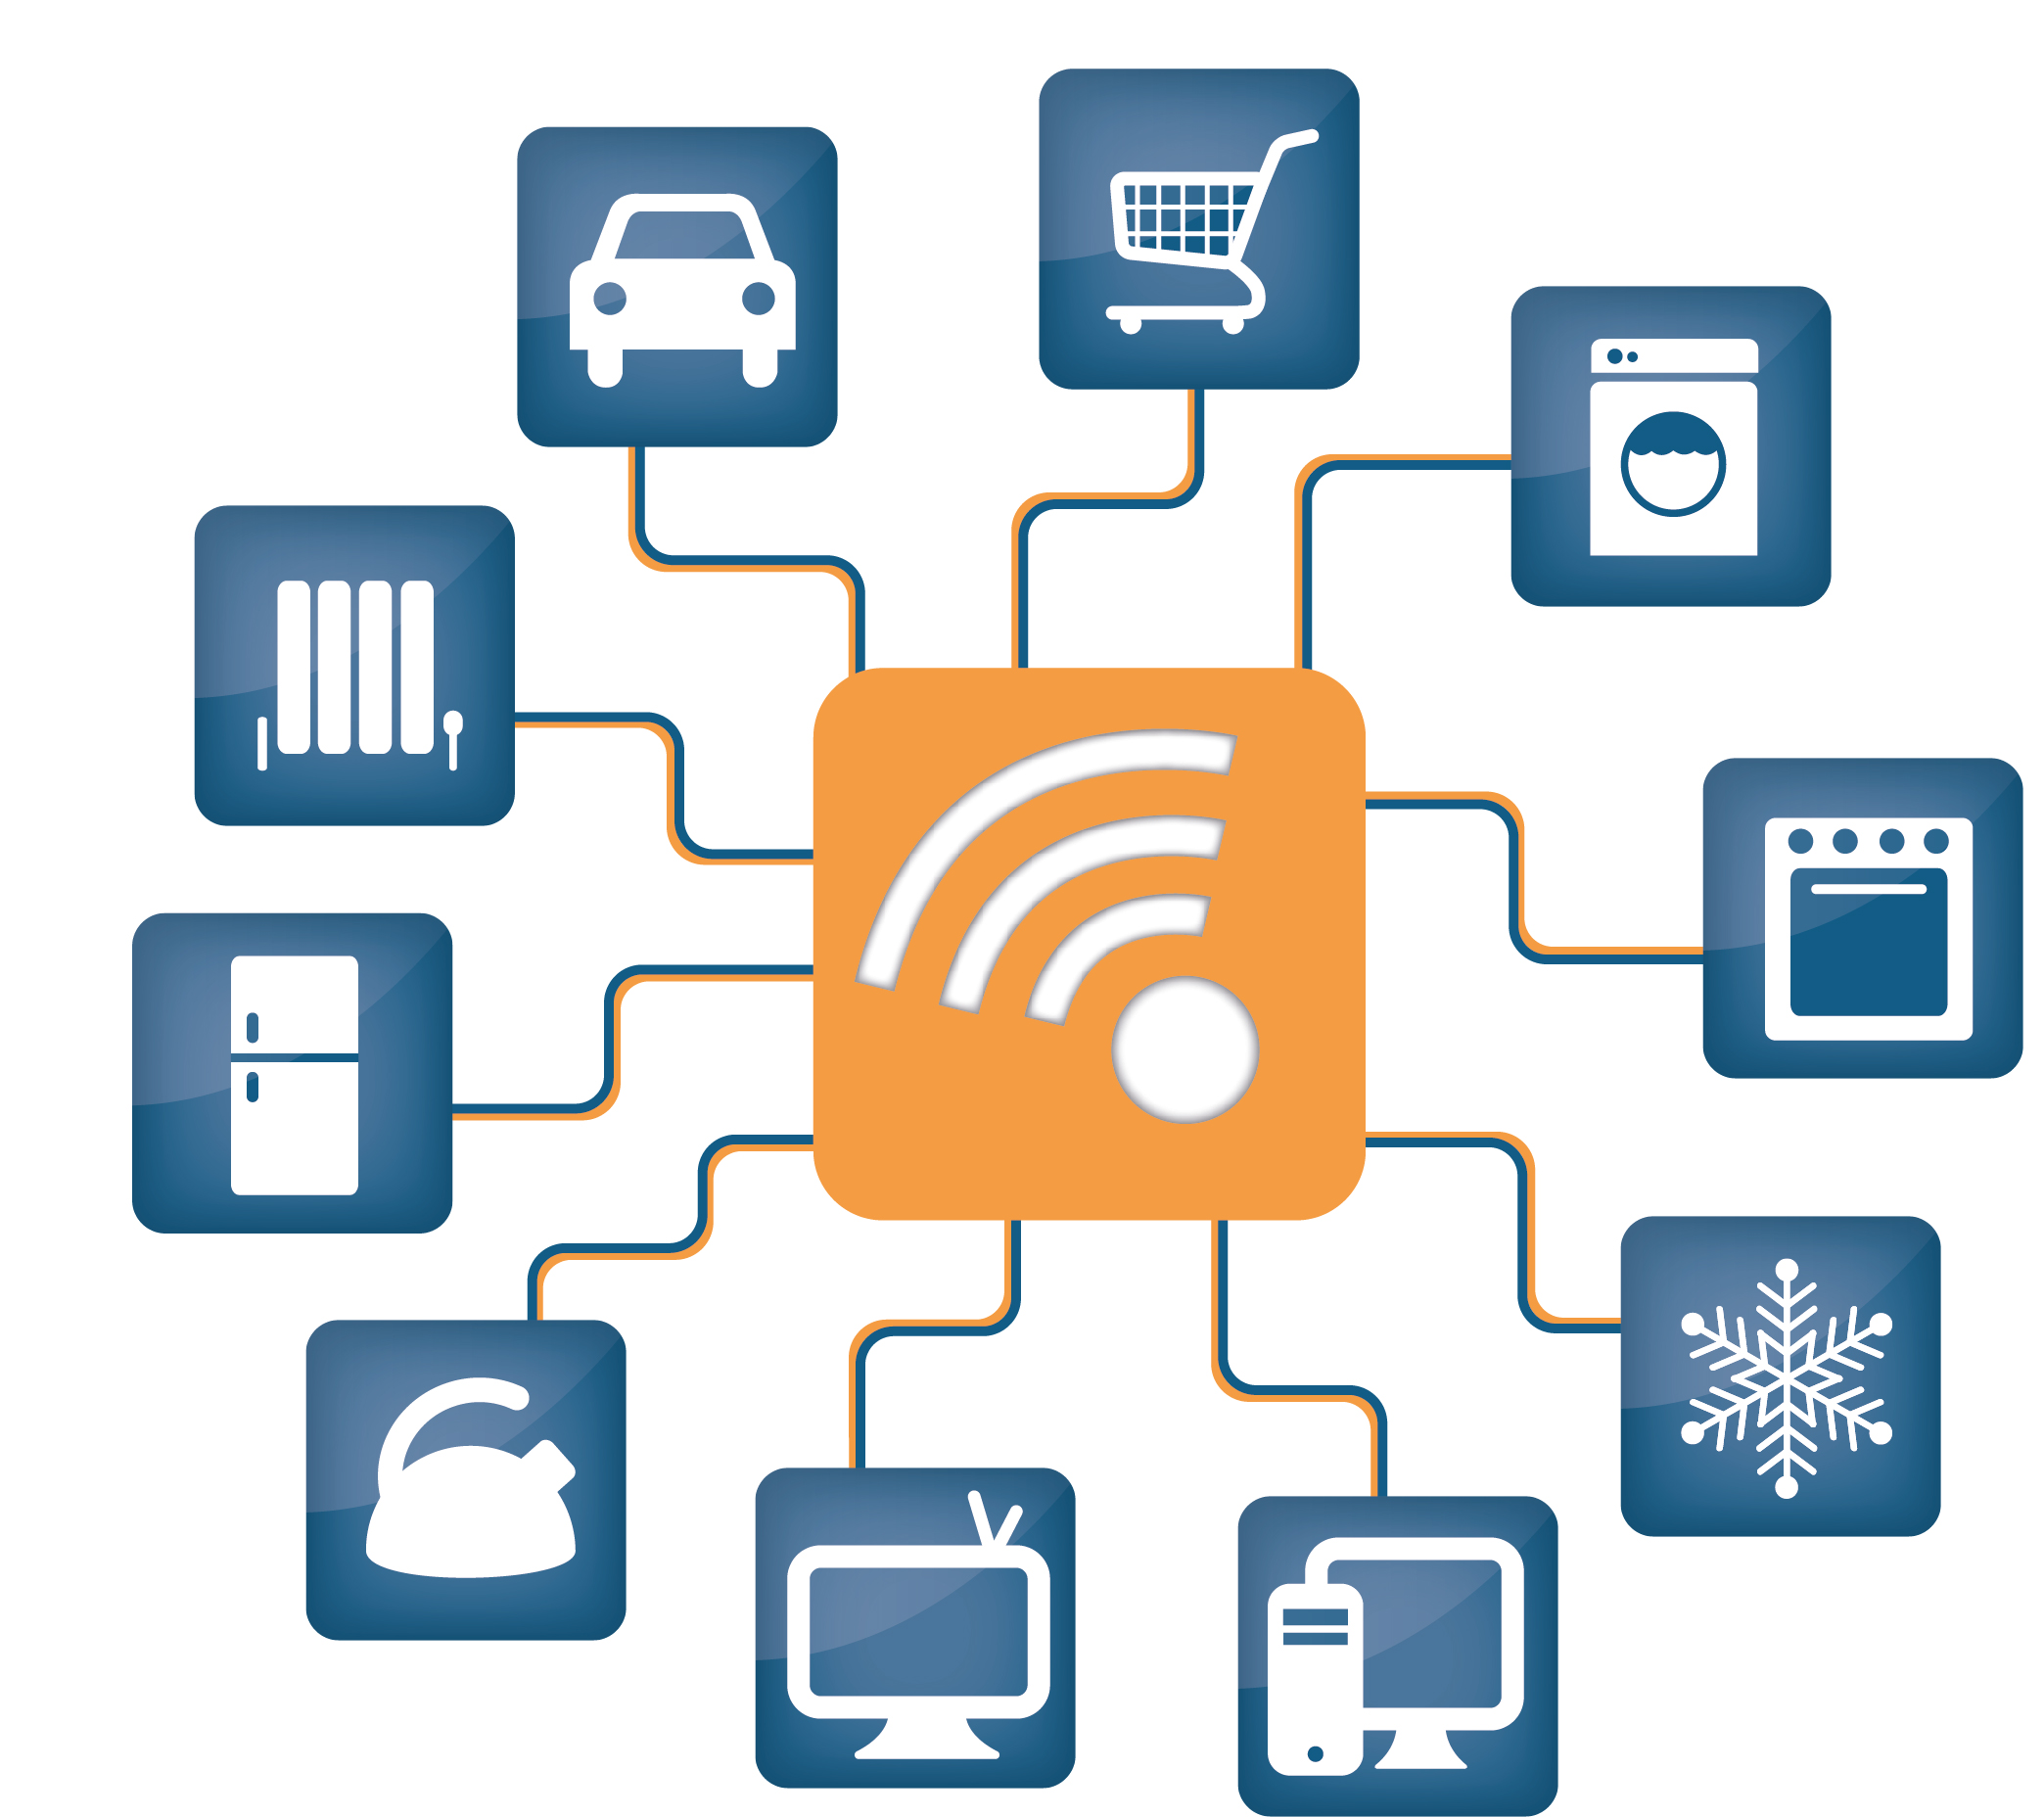
\includegraphics[width=4cm]{figs/Internet-of-Things-4.jpg}
\end{frame}

%------------------------------------------------
\begin{frame}
	\frametitle{IoT's Applications}
	\begin{itemize}
		\item Environmental monitoring
		\item Infrastructure management
		\item Manufacturing
		\item Energy management
		\item Medical and healthcare systems
		\item \textcolor{TextGreen}{\textbf{Building and home automation}}
		\item Transportation
		\item \ldots
	\end{itemize}
\end{frame}

%------------------------------------------------
\begin{frame}
	\frametitle{Building and Home Automation}
	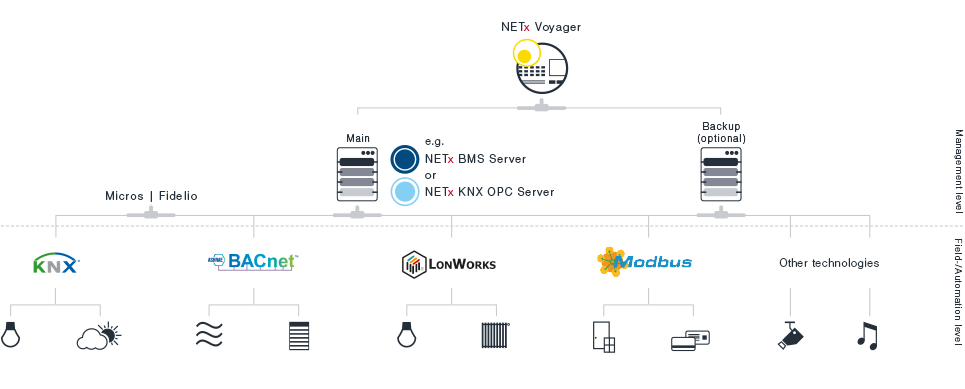
\includegraphics[width=12cm]{figs/voyager-concept.png}
\end{frame}

%------------------------------------------------
\begin{frame}
	\frametitle{Outline}
	\begin{columns}[c]
		\begin{column}{30cm}
			\vspace{.1cm}
			\begin{itemize}
				\justifying
				\item Part I: IoT OS
				\begin{itemize}
					\item \textcolor{LightGray}{Introduction}
					\item IoT Requirements \& Challenges
					\begin{itemize}
						\item[-] R1: Heterogeneous Hardware Constraints
						\item[-] R2: Autonomy 
						\item[-] R3: Programmability
						\item[-] Effect of the requirements on OS
					\end{itemize}
					\item \textcolor{LightGray}{IoT OS}
					\item \textcolor{LightGray}{Existing OSes}
				\end{itemize}
				\item \textcolor{LightGray}{Part II: IoT Protocol Stack}
				\item \textcolor{LightGray}{Part III: IoT Development}
				\item \textcolor{LightGray}{Conclusion}
			\end{itemize}
		\end{column}
	\end{columns}
\end{frame}

%------------------------------------------------
\begin{frame}
	\frametitle{R1: Heterogeneous Hardware Constraints}
	\begin{itemize}
		\justifying
		\item Memory Requirements
		\item CPU Requirements
		\item Limited Features
		\item Platform Support
	\end{itemize}
	\hspace*{7cm} 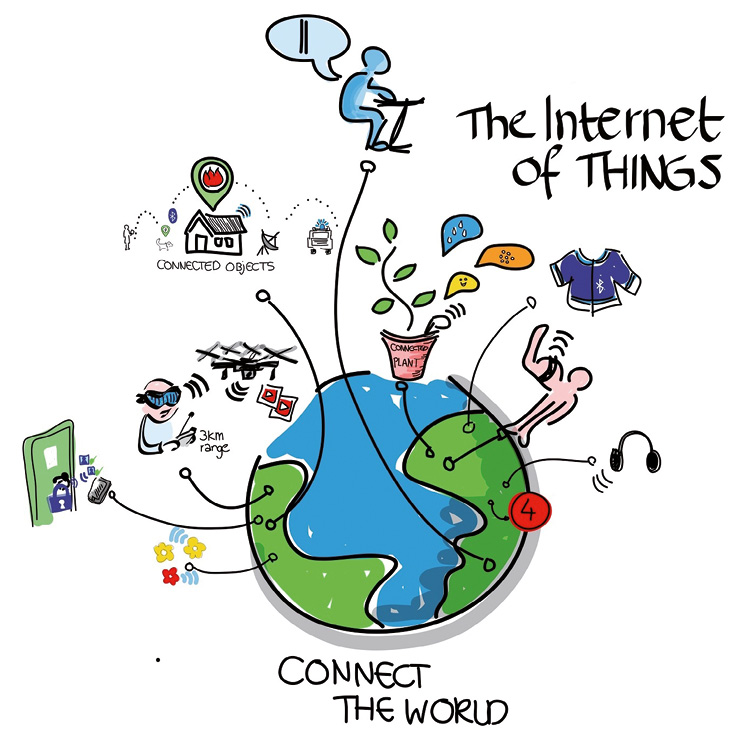
\includegraphics[width=3.5cm]{figs/Internet-of-Things-3.jpg}
\end{frame}

%------------------------------------------------
\begin{frame}
	\frametitle{Memory Requirements}
	\begin{itemize}
		\justifying
		\item Many of typical IoT devices have very little memory (typically between 5kB and some hundreds of megabytes)
		\item This concerns RAM as well as persistent program storage.
	\end{itemize}

	\begin{columns}
	\column{.8\textwidth}
	\begin{block}{\centering\textcolor{darkred}{Effects on OS}}
		\justifying
		\begin{itemize}
			\item Kernel image should be very small
			\item The RAM footprint should be very low
			\item The OS should be modular!
		\end{itemize}
	\end{block}
	\end{columns}

	\vspace{0.5cm}
	\hspace*{7cm} 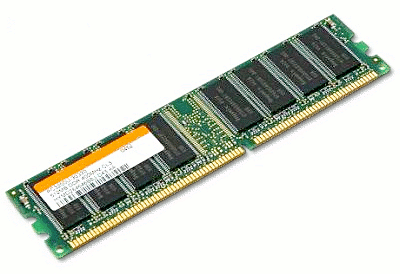
\includegraphics[width=3.5cm]{figs/RAM.png}
\end{frame}

%------------------------------------------------
\begin{frame}
	\frametitle{CPU Requirements}
	\begin{itemize}
		\justifying
		\item Some of the IoT systems are MCU based (instead of CPU)
		\item Some of the MCUs/CPUs in a IoT system will work at a very low clock cycle.
	\end{itemize}

	\begin{columns}
	\column{.8\textwidth}
	\begin{block}{\centering\textcolor{darkred}{Effects on OS}}
		\justifying
		\begin{itemize}
			\item The complexity of OS must be kept very low
			\item Should be scalable, to accommodate a wide range of different classes of devices
		\end{itemize}
	\end{block}
	\end{columns}
	
	\vspace{0.5cm}
	\hspace*{7cm} 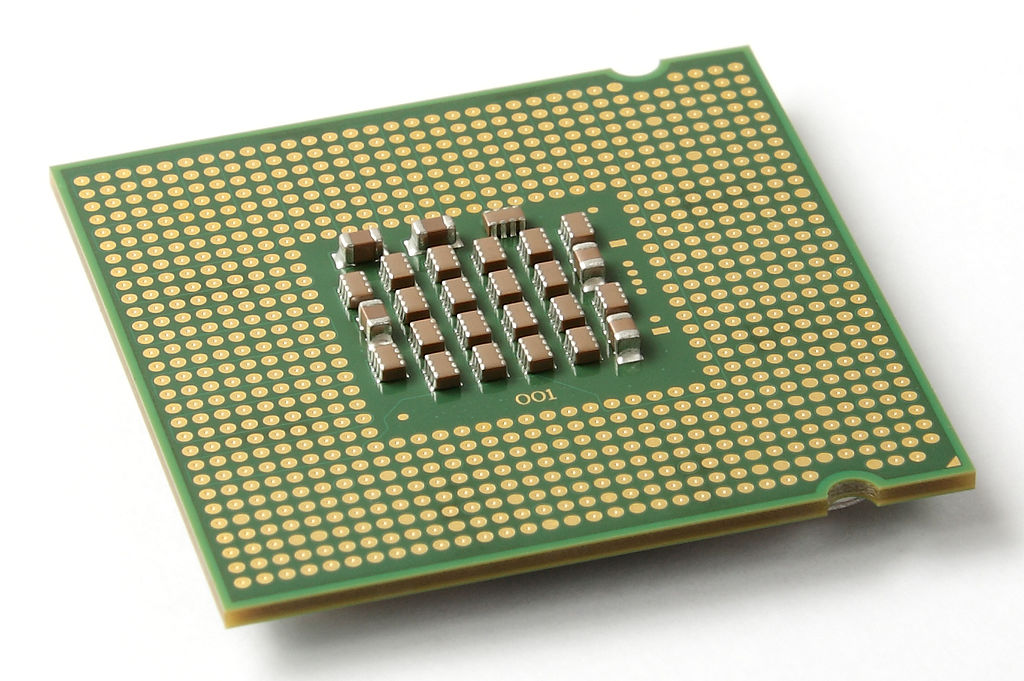
\includegraphics[width=3.5cm]{figs/CPU.jpg}
\end{frame}

%------------------------------------------------
\begin{frame}
	\frametitle{Limited Features}
	\begin{itemize}
		\justifying
		\item IoT's hardware may have not advanced components like a Memory Management Unit (MMU) or a Floating-Point Unit (FPU).
	\end{itemize}

	\begin{columns}
	\column{.8\textwidth}
	\begin{block}{\centering\textcolor{darkred}{Effects on OS}}
		\justifying
		\begin{itemize}
			\item Software for IoT must be able to run on constrained HW
			\item Should be scalable, to accommodate a wide range of different classes of devices
		\end{itemize}
	\end{block}
	\end{columns}
		
	\vspace{0.5cm}
	\hspace*{7cm} 
\includegraphics[width=3.5cm]{figs/Features.jpg}
\end{frame}

%------------------------------------------------
\begin{frame}
	\frametitle{Platform Support}
	\begin{itemize}
		\justifying
		\item IoT platforms may have very limitted resources; e.g., battery, IO, storage, ...
		\item IoT platforms may composed of widly different components
	\end{itemize}

	\begin{columns}
	\column{.8\textwidth}
	\begin{block}{\centering\textcolor{darkred}{Effects on OS}}
		\justifying
		\begin{itemize}
			\item Must be able to leverage the capabilities of less constrained platforms
			\item Should be scalable, to accommodate a wide range of different classes of devices
		\end{itemize}
	\end{block}
	\end{columns}
	\vspace{0.5cm}
	\hspace*{7cm} 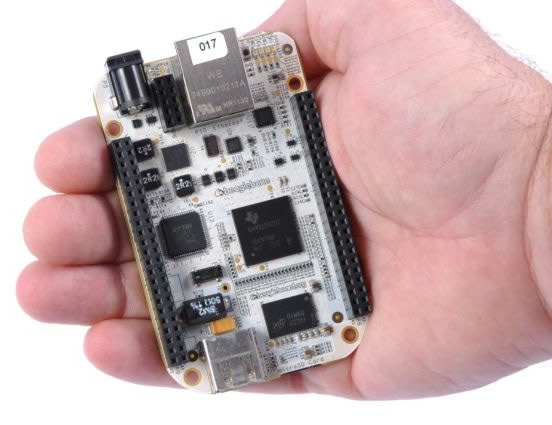
\includegraphics[width=3.5cm]{figs/hw-platform.jpg}
\end{frame}

%------------------------------------------------
\begin{frame}
	\frametitle{R2: Autonomy}
	\begin{columns}[c]
		\begin{column}{30cm}
			\vspace{.1cm}
			\begin{itemize}
				\justifying
				\item Energy Efficiency
				\item Adaptive Network Stack
				\item Reliability
			\end{itemize}
		\end{column}
	\end{columns}
	\hspace*{7cm} 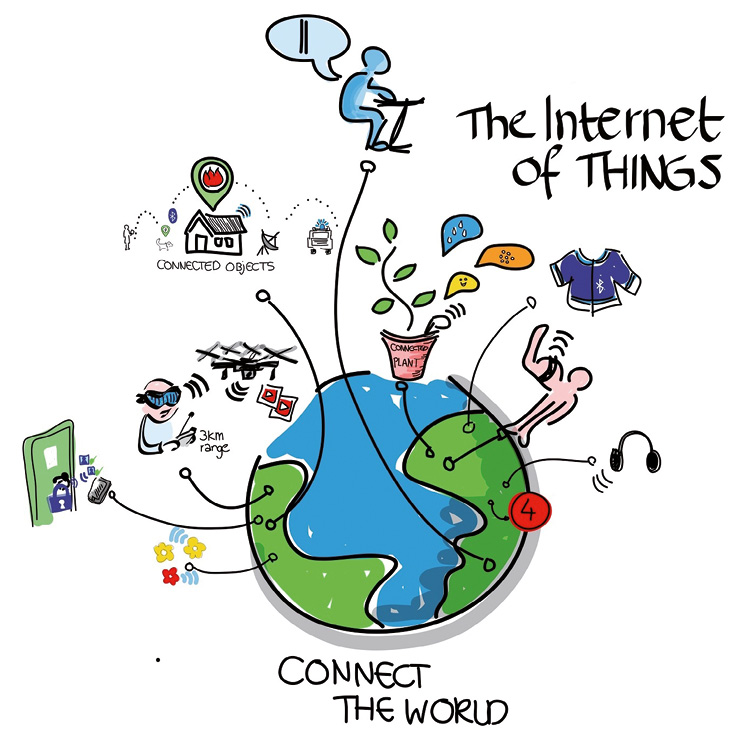
\includegraphics[width=3.5cm]{figs/Internet-of-Things-3.jpg}
\end{frame}

%------------------------------------------------
\begin{frame}
	\frametitle{Energy Efficiency}
	\begin{itemize}
		\justifying
		\item Some IoT nodes are battery powered
		\item Energy efficiency is one the goals of IoT
	\end{itemize}

	\begin{columns}
	\column{.8\textwidth}
	\begin{block}{\centering\textcolor{darkred}{Effects on OS}}
		\justifying
		\begin{itemize}
			\item Must exploit the power saving features of the hardware and allow for large sleep
				cycles as much as possible
		\end{itemize}
	\end{block}
	\end{columns}
	\vspace{0.5cm}
	
	\hspace*{7cm} 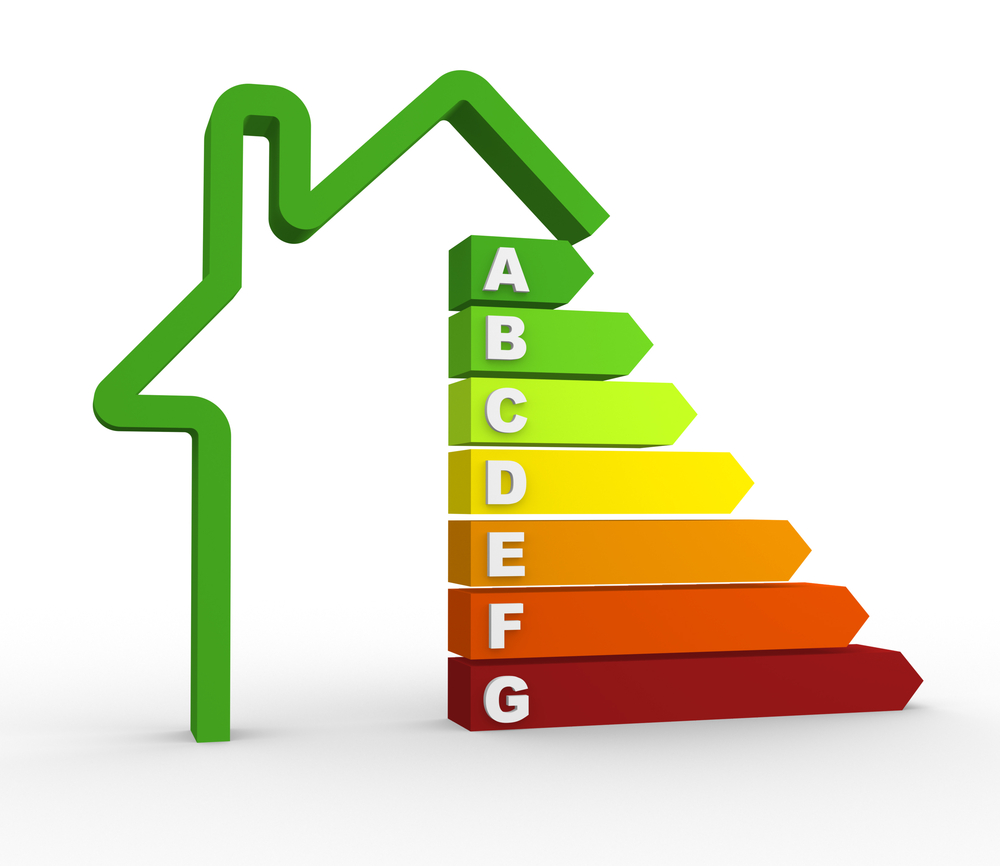
\includegraphics[width=3.5cm]{figs/Energy-efficiency.jpg}
\end{frame}

%------------------------------------------------
\begin{frame}
	\frametitle{Adaptive Network Stack}

	\begin{itemize}
		\justifying
		\item Connectivity is an ingredients part of IoT
		\item IoT is a part of Inernet, TCP/IP based network
		\item IoT can also use its own special protocols 
	\end{itemize}

	\begin{columns}
	\column{.8\textwidth}
	\begin{block}{\centering\textcolor{darkred}{Effects on OS}}
		\justifying
		\begin{itemize}
			\item Should provide full-fledged TCP/IP implementations 
			\item As well as a 6LoWPAN stack aiming for more constrained devices.
			\item It should also be modular in a way that the protocols at each layer can be easily replaced. 
		\end{itemize}
	\end{block}
	\end{columns}
	\vspace{0.5cm}
	
%	\hspace*{3cm} 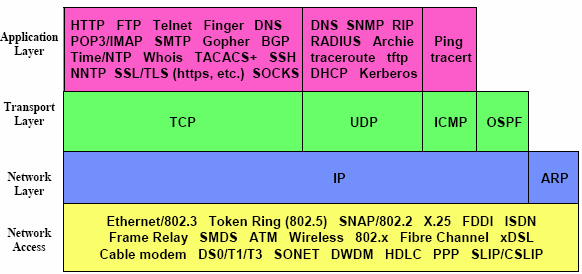
\includegraphics[width=9cm]{figs/tcp-ip-stack.png}
\end{frame}

%------------------------------------------------
\begin{frame}
	\frametitle{Reliability}

	\begin{itemize}
		\justifying
		\item IoT systems are often deployed in critical applications in which physical access is difficult and related to high costs
		\item Timely response is critical in some applications 
	\end{itemize}

	\begin{columns}
	\column{.8\textwidth}
	\begin{block}{\centering\textcolor{darkred}{Effects on OS}}
		\justifying
		\begin{itemize}
			\item System must be robust and thus that the operating system should run very reliably
			\item Real-Time OS in some applications
		\end{itemize}
	\end{block}
	\end{columns}
	\vspace{0.5cm}
		
	\hspace*{7cm} 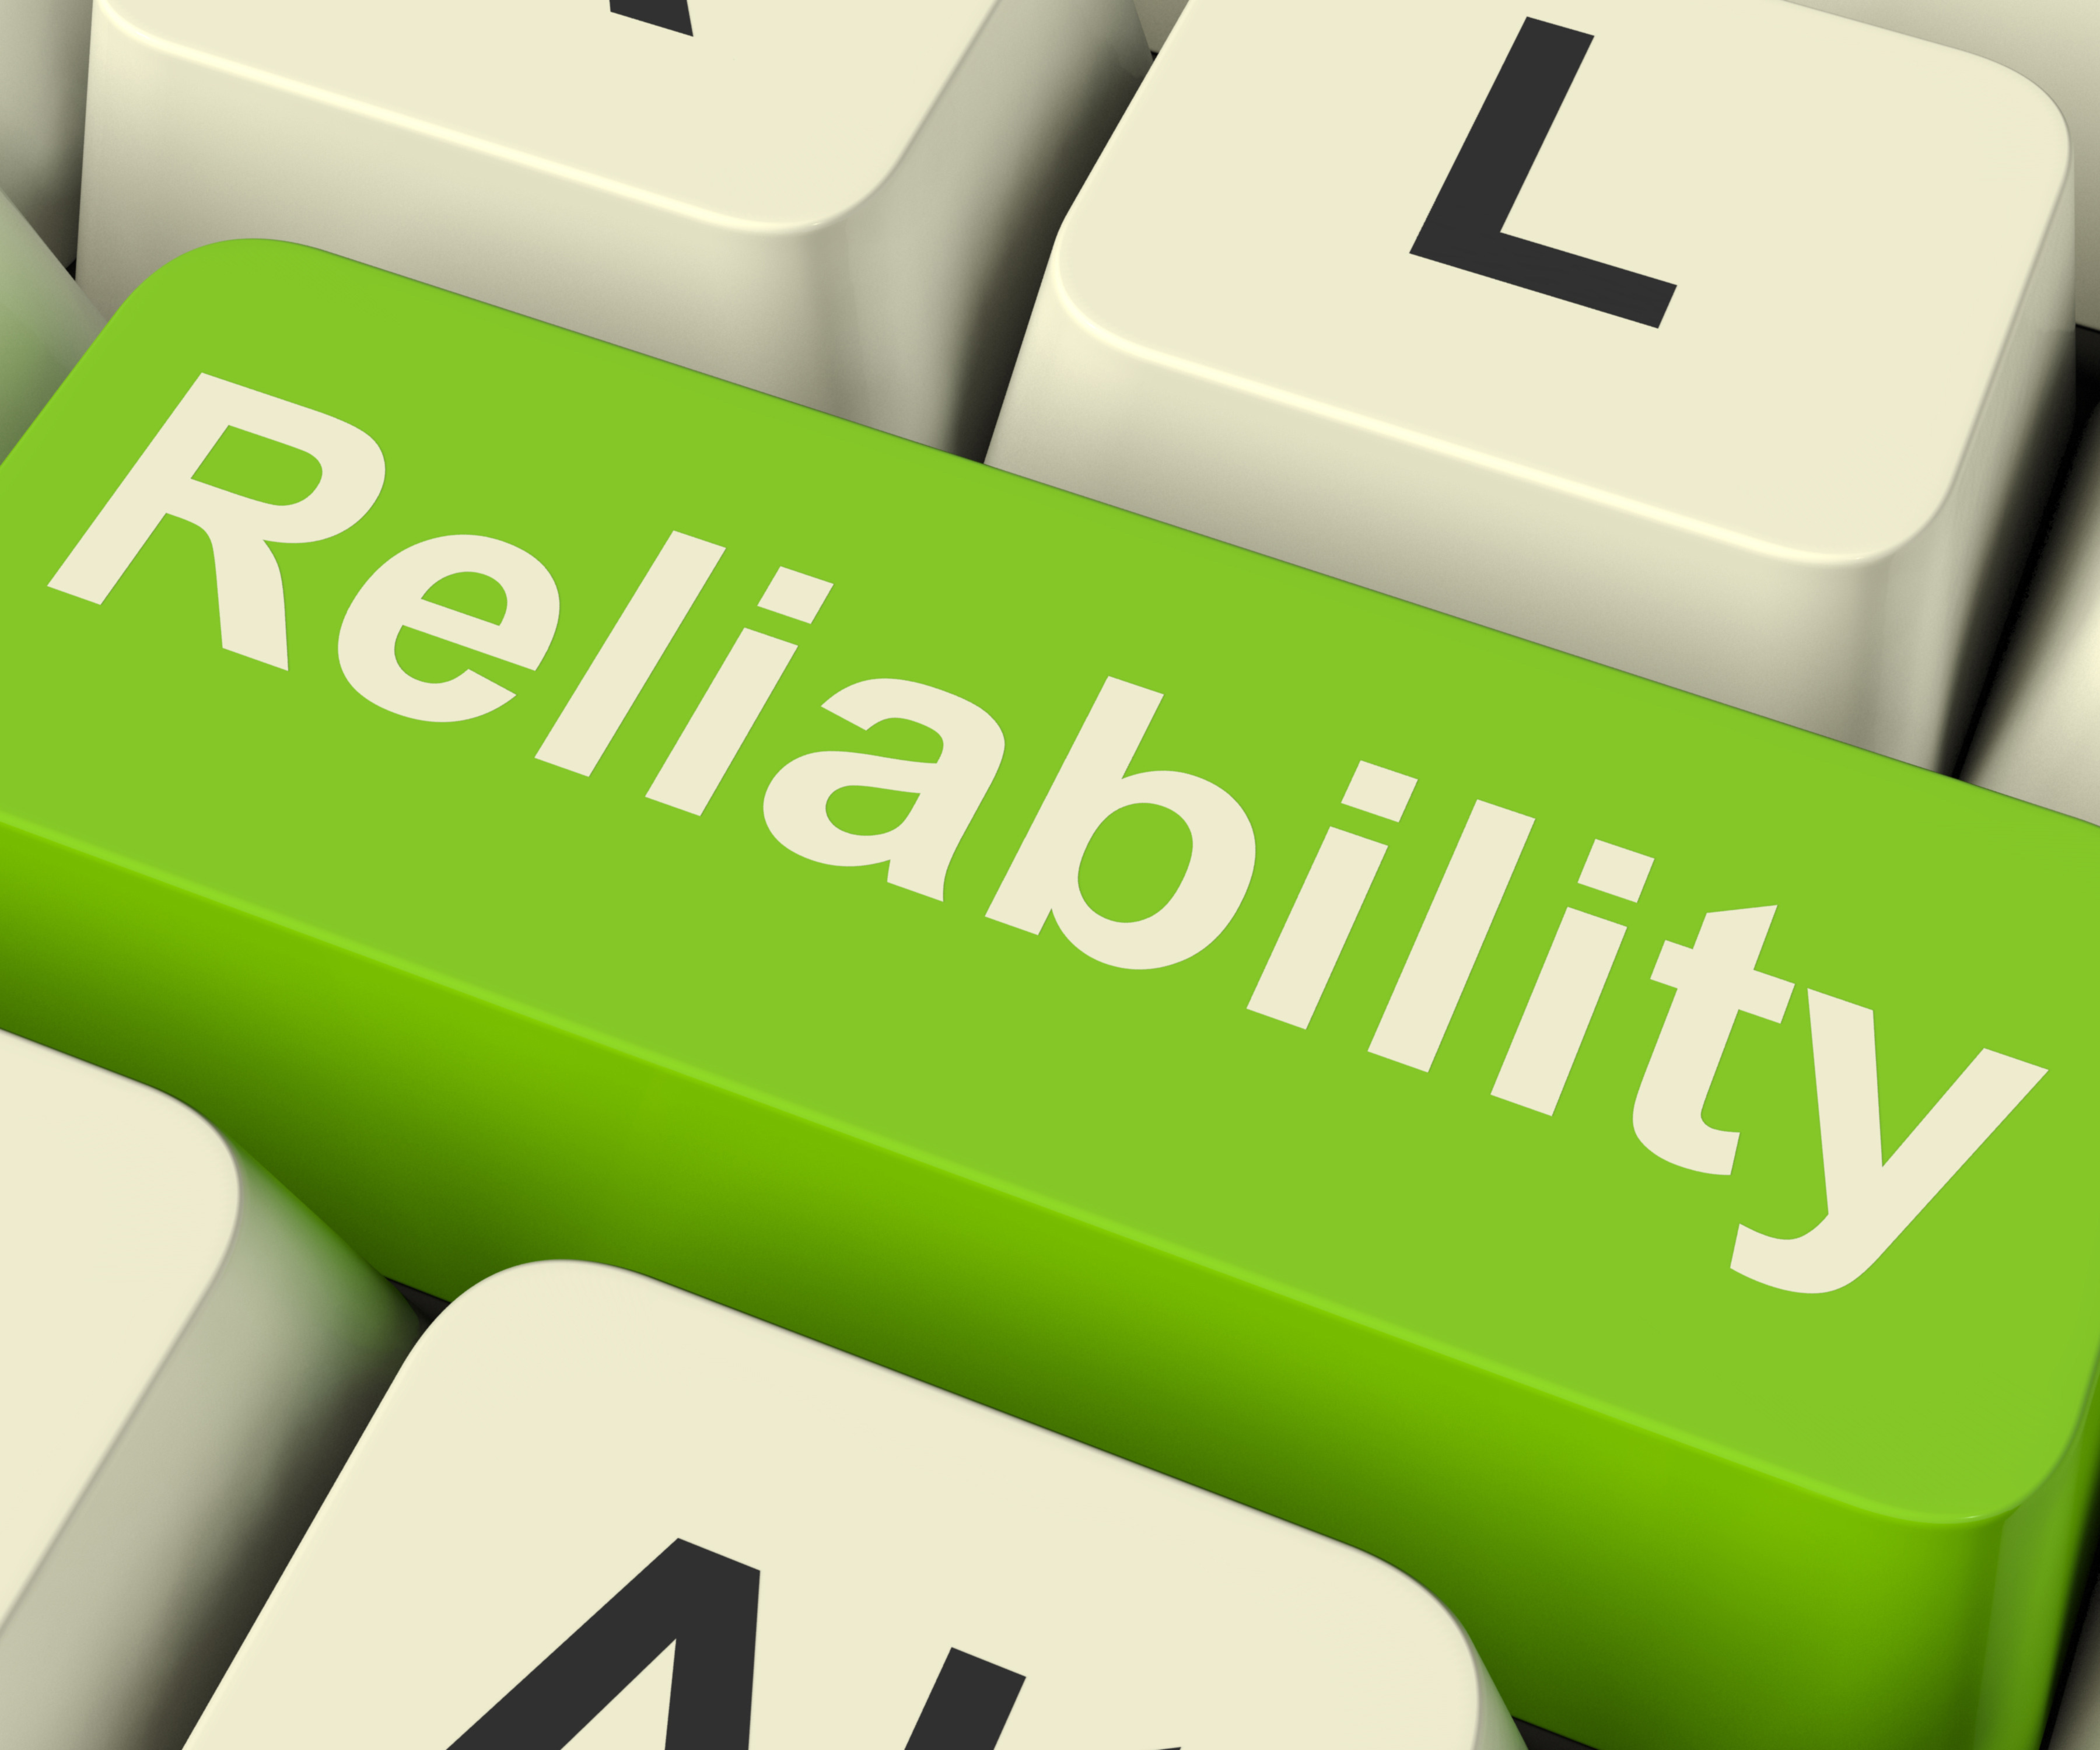
\includegraphics[width=3.5cm]{figs/reliability.jpg}
\end{frame}

%------------------------------------------------
\begin{frame}
	\frametitle{R3: Programmability}
	\begin{columns}[c]
		\begin{column}{30cm}
			\vspace{.1cm}
			\begin{itemize}
				\justifying
				\item Standard API
				\item Standard Programming Languages
			\end{itemize}
		\end{column}
	\end{columns}
	\hspace*{7cm} 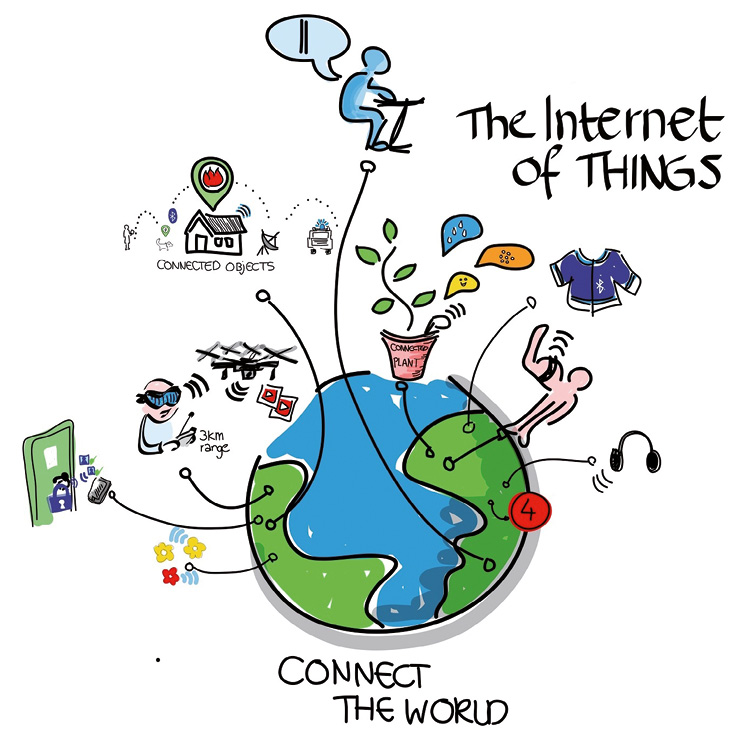
\includegraphics[width=3.5cm]{figs/Internet-of-Things-3.jpg}
\end{frame}

%------------------------------------------------
\begin{frame}
	\frametitle{Standard API \& Programming Languages}

	\begin{itemize}
		\justifying
		\item Need for SW development for IoT systems
		\item Porting of existing software on IoT systems
	\end{itemize}

	\begin{columns}
	\column{.8\textwidth}
	\begin{block}{\centering\textcolor{darkred}{Effects on OS}}
		\justifying
		\begin{itemize}
			\item Standard programming interface such as POSIX or STL should be provided
			\item Support for standard high level programming languages, e.g., C \& C++, is vital.			
		\end{itemize}
	\end{block}
	\end{columns}
	\vspace{0.5cm}

	\hspace*{7cm} 
\includegraphics[width=3.5cm]{figs/ieee-posix-certified.jpg}
\end{frame}

\iffalse
%------------------------------------------------
\begin{frame}
	\frametitle{IoT Challenges}
	\colorbox{green}{\textcolor{red}{References are useful \& needed}}	
	\begin{columns}[c]
		\begin{column}{30cm}
			\vspace{.1cm}
			\begin{itemize}
				\justifying
				\item Heterogeneous hardware
				\item Slow CPU, often no FPU
				\item Little memory, often no MMU
				\item Limited energy resources
				\item Robustness and self-organization
				\item Real-Time requirements
			\end{itemize}
		\end{column}
	\end{columns}
	\hspace*{7cm} 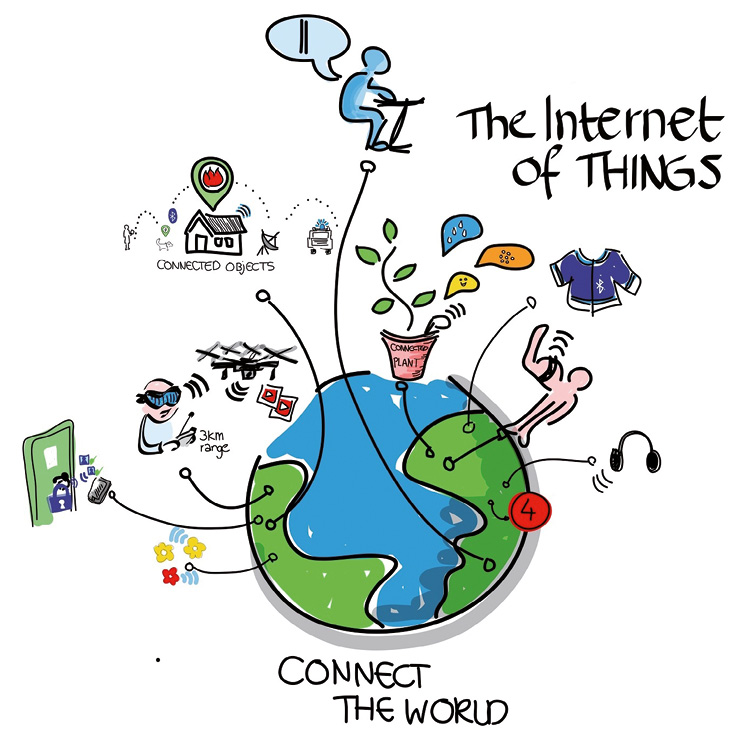
\includegraphics[width=3.5cm]{figs/Internet-of-Things-3.jpg}
\end{frame}

%------------------------------------------------
\begin{frame}
	\frametitle{Effect of the requirements on OS}
	\begin{columns}[c]
		\begin{column}{30cm}
			\vspace{.1cm}
			\begin{itemize}
				\justifying
				\item \textcolor{TextOrange}{Scalable}, to accommodate a wide range of different
				 classes of devices
				\item \textcolor{TextGreen}{Modular}, so you can choose only the components you\\
				need to meet tight RAM requirements
				\item \textcolor{TextOrange}{Connected}, so you can move data in and out of the\\
				device via Wi-Fi, Ethernet, USB, or Bluetooth.
				\item \textcolor{TextGreen}{Reliable}, so your device can be certified for safety-critical
				applications
			\end{itemize}
		\end{column}
	\end{columns}
\end{frame}
\fi
%------------------------------------------------
\begin{frame}
	\frametitle{Outline}
	\begin{columns}[c]
		\begin{column}{30cm}
			\vspace{.1cm}
			\begin{itemize}
				\justifying
				\item Part I: IoT OS
				\begin{itemize}
					\item \textcolor{LightGray}{Introduction}
					\item \textcolor{LightGray}{IoT Requirements \& Challenges}
					\item {IoT OS}
					\begin{itemize}
						\item[-] General OS vs IoT OS
						\item[-] What are the main requirements in IoT OS
						\item[-] What are the main components in IoT OS
				\end{itemize}
					\item \textcolor{LightGray}{Existing OSes}
				\end{itemize}
				\item \textcolor{LightGray}{Part II: IoT Protocol Stack}
				\item \textcolor{LightGray}{Part III: IoT Development}
				\item \textcolor{LightGray}{Conclusion}
			\end{itemize}
		\end{column}
	\end{columns}
\end{frame}

%------------------------------------------------
\begin{frame}
	\frametitle{General OS}
	\vspace{.5cm}
	\begin{center}
	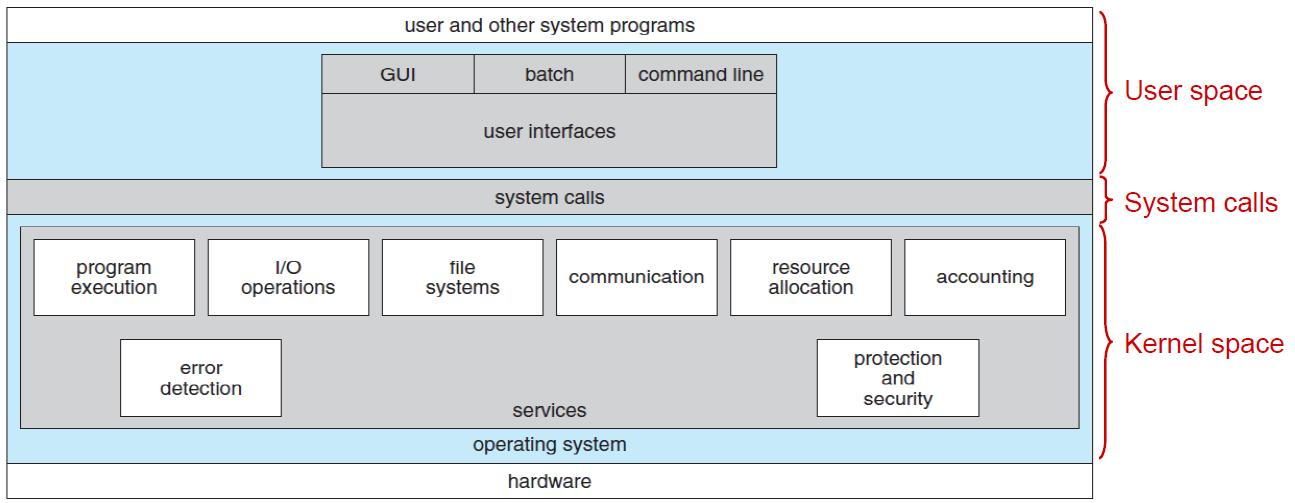
\includegraphics[width=10cm]{figs/os-components.jpg}
	\end{center}
\end{frame}

%------------------------------------------------
\begin{frame}
	\frametitle{Linux Kernel Architecture (Simple Version)}
	\begin{center}
	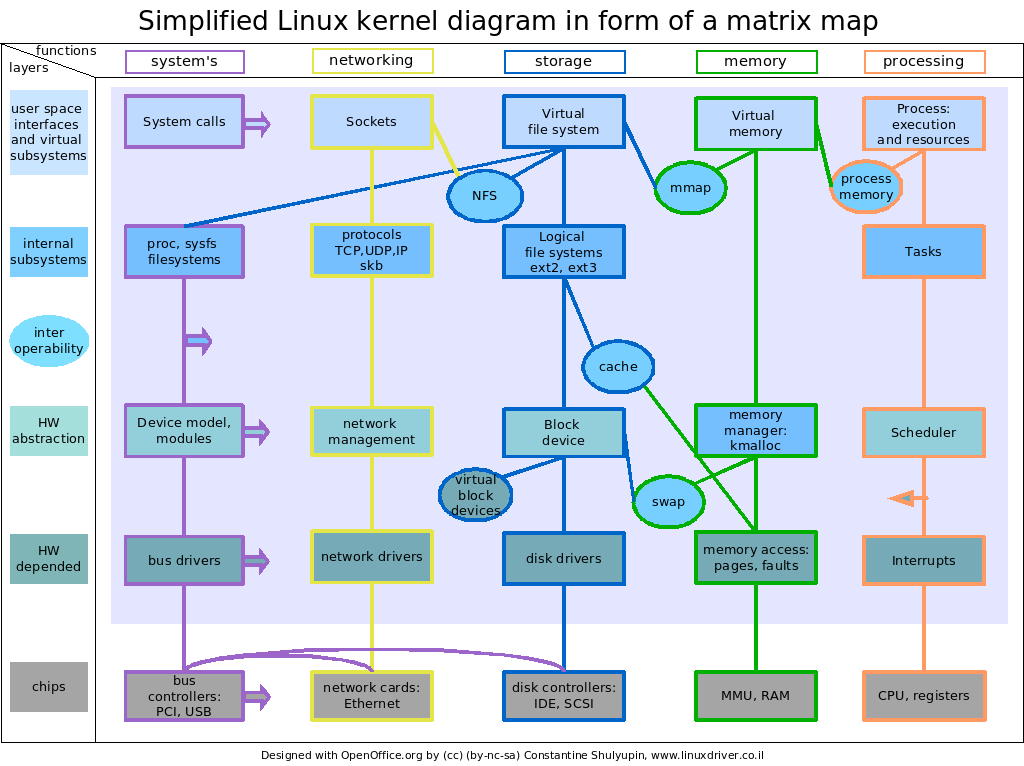
\includegraphics[width=10cm]{figs/Simple_Linux_kernel_diagram.png}	
	\end{center}
\end{frame}

%------------------------------------------------
\begin{frame}
	\frametitle{Linux Kernel Architecture (Almost Complete Version)}
	\begin{center}
	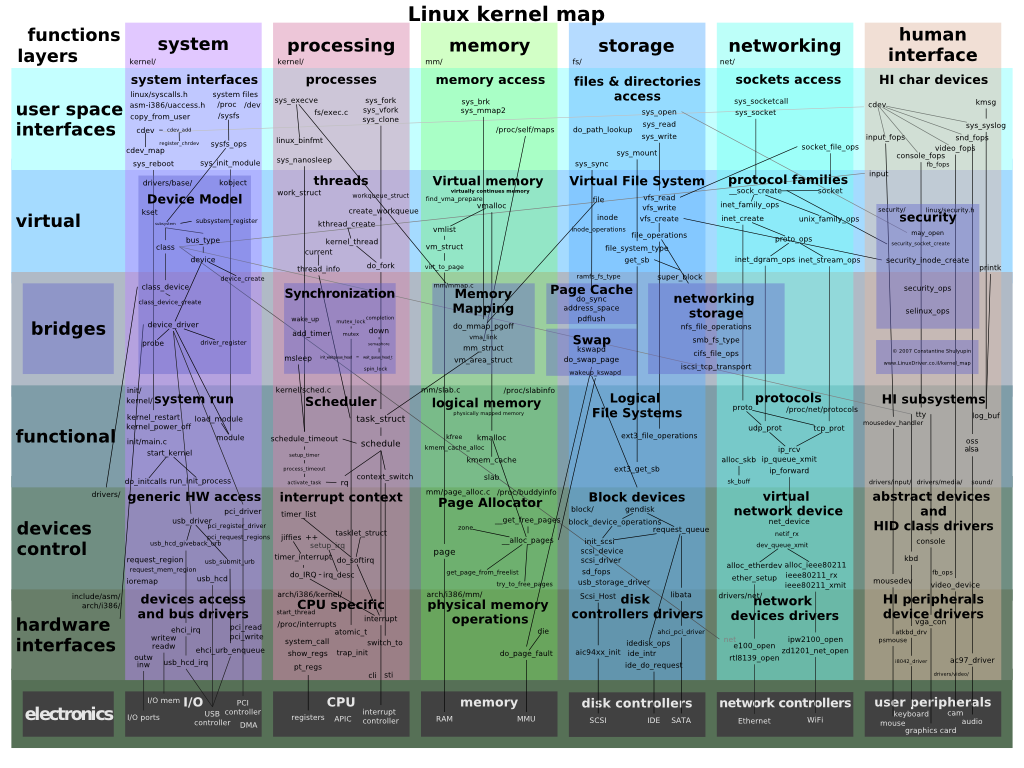
\includegraphics[width=10cm]{figs/Complex_Linux_kernel_map.png}	
	\end{center}
\end{frame}

%------------------------------------------------
\begin{frame}
	\frametitle{IoT OS/Kernel}
	\begin{itemize}
		\item Much more simpler than general OS/Kernel
		\item Do we need?!
		\begin{itemize}
			\item Human interface
			\item Full wide-range storage support
			\item Virtual memory
			\item Full traditional protocol stack 
		\end{itemize}
		\item Its own requirements, remarkably
		\begin{itemize}
			\justifying
			\item IoT Protocol Stack Support
			\item Low Complexity
			\item Efficient Memory Managing
			\item Real-Time Task Scheduling
		\end{itemize}			
	\end{itemize}
\end{frame}

%------------------------------------------------
\begin{frame}
	\frametitle{IoT OS Example: ARM's mbed}
	\begin{center}
	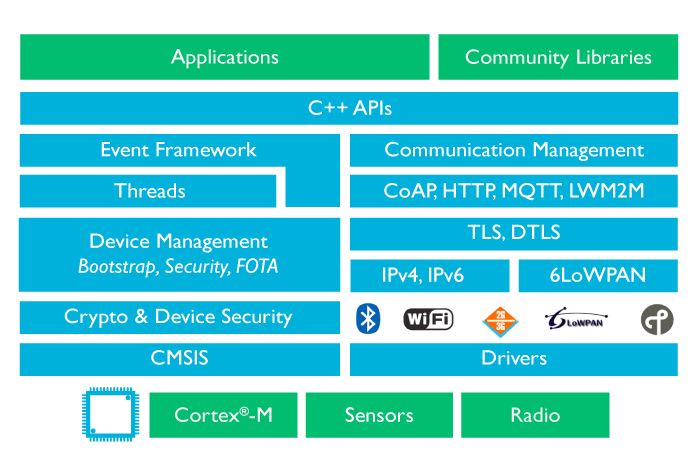
\includegraphics[width=10cm]{figs/mbed-components.png}	
	\end{center}
\end{frame}

%------------------------------------------------
\begin{frame}
	\frametitle{Outline}
	\begin{columns}[c]
		\begin{column}{30cm}
			\vspace{.1cm}
			\begin{itemize}
				\justifying
				\item Part I: IoT OS
				\begin{itemize}
					\item \textcolor{LightGray}{Introduction}
					\item \textcolor{LightGray}{IoT Requirements \& Challenges}
					\item \textcolor{LightGray}{IoT OS}
					\item {Existing OSes}
					\begin{itemize}
						\item[-] OS Classification
						\item[-] Overview of Open Source OSes
						\item[-] Overview of Closed Source OSes
						\item[-] Why Not Linux?
					\end{itemize}
				\end{itemize}
				\item \textcolor{LightGray}{Part II: IoT Protocol Stack}
				\item \textcolor{LightGray}{Part III: IoT Development}
				\item \textcolor{LightGray}{Conclusion}
			\end{itemize}
		\end{column}
	\end{columns}
\end{frame}

%------------------------------------------------
\begin{frame}
	\frametitle{OS Classification}
	\begin{itemize}
		\justifying
		\item Single-tasking vs. Multi-tasking
			\begin{itemize}
				\item<2-> Multi-tasking in IoT OS
			\end{itemize}
		\item Single-user vs. Multi-user
			\begin{itemize}
				\item<2-> Single-user in IoT OS
			\end{itemize}		
		\item Monolithic vs. Microkernel
			\begin{itemize}
				\item<2-> Both can be used in IoT OS
			\end{itemize}		
		\item Process model vs. Thread model
			\begin{itemize}
				\item<2-> Thread in IoT OS, since No MMU \& Realtimeness
			\end{itemize}					
		\item Open source vs. Commercial
			\begin{itemize}
				\item<2-> Both are available in IoT OS market
			\end{itemize}				
	\end{itemize}
\end{frame}


%------------------------------------------------
\begin{frame}
	\frametitle{Overview of Open Source OSes}
	\begin{columns}[c]
		\begin{column}{30cm}
			\vspace{.1cm}
			\begin{itemize}
				\justifying
				\item \textcolor{blue}{\href{http://www.freertos.org}{FreeRTOS}}
				\item \textcolor{blue}{\href{http://www.riot-os.org}{RIOT}}
				\item \textcolor{blue}{\href{http://www.contiki-os.org}{Contiki}}
				\item TinyOS
				\item Embedded Linux
				\item \textcolor{blue}{\href{http://www.openwsn.org}{OpenWSN}}
			\end{itemize}
		\end{column}
	\end{columns}
	\vspace{.5cm}
	\hspace*{5.5cm} 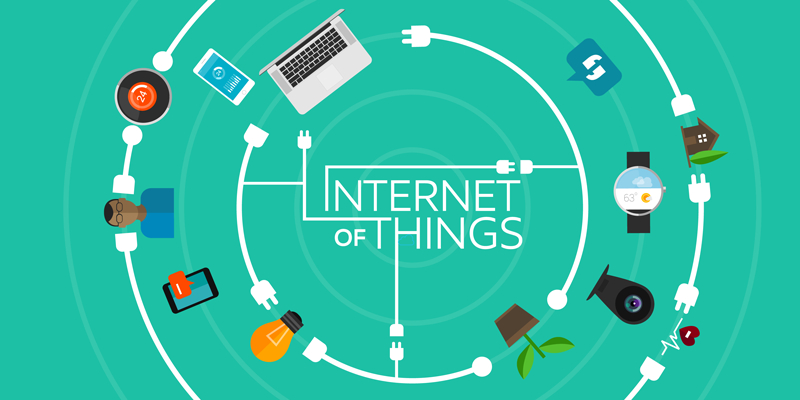
\includegraphics[width=5cm]{figs/Internet-of-Things-2.jpg}
\end{frame}

%------------------------------------------------
\begin{frame}
	\frametitle{FreeRTOS}
	\begin{itemize}
		\justifying
		\item Owned, developed, maintained, distributed and supported by Real Time Engineers Ltd
			\begin{itemize}
				\item It claims that is market leading RTOS
			\end{itemize}
		\item FreeRTOS is designed to be \textcolor{TextOrange}{small}
		and \textcolor{TextOrange}{simple}.
		\begin{itemize}
			\item ROM/Flash footprint from 5K to 12K bytes
			\item RAM footprint $\approx$ 250 bytes,
		\end{itemize}
		\item The kernel itself consists of only three or four C files.
		\begin{itemize}
			\item It provides methods for multiple threads or tasks, mutexes, semaphores and software timers.		
		\end{itemize}
		\item Key features are \textcolor{TextGreen}{very small memory footprint},
		\textcolor{TextGreen}{low overhead}, and \textcolor{TextGreen}{very fast execution}.
	\end{itemize}

	\vspace{.5cm}
	\hspace*{5.5cm} 
\includegraphics[width=5cm]{figs/freertos-logo.jpg}	
\end{frame}

%------------------------------------------------
\begin{frame}
	\frametitle{RIOT}
	\begin{itemize}
		\item Is an operating system for Internet of Things (IoT) devices.
		\item RIOT is a \textcolor{TextOrange}{real-time} \textcolor{TextOrange}{multi-threading} operating system.
		\item RIOT implements a \textcolor{TextGreen}{microkernel} architecture
		\item RIOT is based on design objectives including:
		\begin{itemize}
			\item Energy-Efficiency
			\item High degree of modularity
			\item Reliability
			\item Real-Time Capabilities
			\begin{itemize}
				\item[-] a preemptive, tickless scheduler with priorities
			\end{itemize}
			\item Small Memory Footprint
			\item API independent of the HW (partial POSIX) + Wiselib support
			\item Networking: IPv6, UDP, 6LoWPAN, ...
		\end{itemize}
	\end{itemize}
	\vspace{.05cm}
	\hspace*{7cm} 
\includegraphics[width=5cm]{figs/riot-logo.png}
\end{frame}

%------------------------------------------------
\begin{frame}
	\frametitle{Contiki}
	\begin{columns}[c]
		\begin{column}{30cm}
			\vspace{.1cm}
			\begin{itemize}
				\justifying
				\item Contiki is an open source operating system for \textcolor{TextOrange}{networked},\\
				\textcolor{TextOrange}{memory-constrained} systems
				\item Contiki provides three network mechanisms:
				\begin{itemize}
					\justifying
					\item The uIP stack, which provides IPv4 networking,
					\item The uIPv6 stack, which provides IPv6 networking,
					\item The Rime stack, which is a set of custom lightweight networking protocols\\
					designed specifically for low-power wireless networks.
				\end{itemize}
			\end{itemize}
		\end{column}
	\end{columns}
	\vspace{.5cm}
	\hspace*{5.5cm} 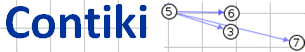
\includegraphics[width=5cm]{figs/contiki-logo.png}
\end{frame}

%------------------------------------------------
\begin{frame}
	\frametitle{TinyOS}
	\begin{itemize}
		\item TinyOS is a \textcolor{TextOrange}{component-based} operating system and platform targeting wireless sensor networks.
		\begin{itemize}
			\item Components are connected to each other using interfaces
			\item Components for common abstractions such as packet communication, routing, sensing, actuation and storage
		\end{itemize}
		\item TinyOS is an embedded operating system written in the \textcolor{TextOrange}{nesC programming language} as a set of cooperating tasks and processes.
	\end{itemize}
	\vspace{.5cm}
	\hspace*{5.5cm} 
\includegraphics[width=5cm]{figs/tinyos-logo.jpg}
\end{frame}

%------------------------------------------------
\begin{frame}
	\frametitle{Embedded Linux}
	\begin{columns}[c]
		\begin{column}{30cm}
			\vspace{.1cm}
			\begin{itemize}
				\justifying
				\item Embedded Linux is created using OpenEmbedded,\\
				the build framework for embedded Linux.
				\item OpenEmbedded offers a best-in-class cross-compile environment.
			\end{itemize}
		\end{column}
	\end{columns}
	\vspace{.5cm}
	\hspace*{5.5cm} 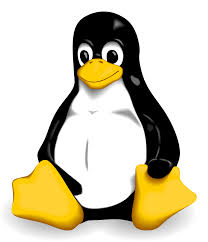
\includegraphics[width=5cm]{figs/linux-logo.jpeg}
\end{frame}

%------------------------------------------------
\begin{frame}
	\frametitle{OpenWSN}
	\begin{itemize}
		\item TProvides open-source implementations of a complete protocol stack based on Internet of Things standards, on a variety of software and hardware platforms.
		\item Enables ultra-low power and highly reliable mesh networks which are fully integrated into the Internet
		\item Protocols
				\begin{itemize}
					\item IEEE802.15.4e
					\item IETF 6TiSCH 
					\item IETF 6LoWPAN
					\item IETF ROLL
					\item RPL
					\item ...
				\end{itemize}
			\end{itemize}
	\hspace*{5.5cm} 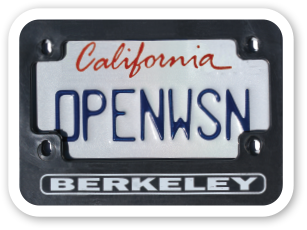
\includegraphics[width=4cm]{figs/openwsn-logo.png}
\end{frame}

%------------------------------------------------
\begin{frame}
	\frametitle{Comparison}
	\begin{columns}[c]
		\begin{column}{30cm}
			\hspace{0.9cm}
			\begin{tabular}{| c | c | c | c | c |}
				\hline
				OS & Min RAM & Min ROM & C Support & C++ Support \\ \hline
				Contiki & $< 2kB$ & $< 30kB$ & \textcolor{TextOrange}{Partial support} &
				\textcolor{red}{No support} \\ \hline
				Tiny OS & $< 1kB$ & $< 4kB$ & \textcolor{red}{No support} &
				\textcolor{red}{No support} \\ \hline
				Linux & $\sim 1MB$ & $\sim 1MB$ & \textcolor{TextGreen}{Full support} &
				\textcolor{TextGreen}{Full support} \\ \hline
				RIOT & $\sim 1.5kB$ & $\sim 5kB$ & \textcolor{TextGreen}{Full support} &
				\textcolor{TextGreen}{Full support} \\ \hline
			\end{tabular}
		\end{column}
	\end{columns}
	\vspace{.5cm}
	\hspace*{1cm}
	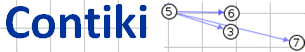
\includegraphics[width=2cm]{figs/contiki-logo.png}
	\hspace*{.5cm}
	
\includegraphics[width=2cm]{figs/tinyos-logo.jpg}
	\hspace*{.5cm}
	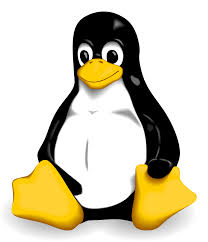
\includegraphics[width=2cm]{figs/linux-logo.jpeg}
	\hspace*{.5cm}
	
\includegraphics[width=2cm]{figs/riot-logo.png}
\end{frame}

%------------------------------------------------
\begin{frame}
	\frametitle{Comparison}
	\begin{columns}[c]
		\begin{column}{30cm}
			\hspace{0.9cm}
			\begin{tabular}{| c | c | c | c |}
				\hline
				OS & Multi-Threading & Modularity & Real-Time \\ \hline
				Contiki & \textcolor{TextOrange}{Partial support} &
				\textcolor{TextOrange}{Partial support} &
				\textcolor{TextOrange}{Partial support} \\ \hline
				Tiny OS & \textcolor{TextOrange}{Partial support} &
				\textcolor{red}{No support} &
				\textcolor{red}{No support} \\ \hline
				Linux & \textcolor{TextGreen}{Full support} &
				\textcolor{TextOrange}{Partial support} &
				\textcolor{TextOrange}{Partial support} \\ \hline
				RIOT & \textcolor{TextGreen}{Full support} &
				\textcolor{TextGreen}{Full support} &
				\textcolor{TextGreen}{Full support} \\ \hline
			\end{tabular}
		\end{column}
	\end{columns}
	\vspace{.5cm}
	\hspace*{1cm}
	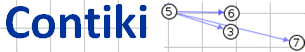
\includegraphics[width=2cm]{figs/contiki-logo.png}
	\hspace*{.5cm}
	
\includegraphics[width=2cm]{figs/tinyos-logo.jpg}
	\hspace*{.5cm}
	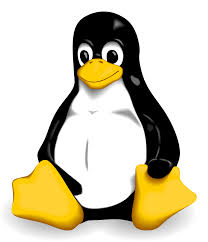
\includegraphics[width=2cm]{figs/linux-logo.jpeg}
	\hspace*{.5cm}
	
\includegraphics[width=2cm]{figs/riot-logo.png}
\end{frame}

%------------------------------------------------
\begin{frame}
	\frametitle{Operating Systems Availability}
	\begin{columns}[c]
		\begin{column}{30cm}
			\hspace{0.9cm}
			\begin{tabular}{| c | c | c | c |}
				\hline
				OS & Wsn430 Node & M3 Node & A8 Node \\ \hline
				Contiki & \textcolor{TextGreen}{Full support} &
				\textcolor{TextGreen}{Full support} &
				\textcolor{red}{No support} \\ \hline
				Tiny OS & \textcolor{TextGreen}{Full support} &
				\textcolor{red}{No support} &
				\textcolor{red}{No support} \\ \hline
				Linux & \textcolor{red}{No support} &
				\textcolor{red}{No support} &
				\textcolor{TextGreen}{Full support} \\ \hline
				RIOT & \textcolor{TextGreen}{Full support} &
				\textcolor{TextGreen}{Full support} &
				\textcolor{red}{No support} \\ \hline
			\end{tabular}
		\end{column}
	\end{columns}
	\vspace{.5cm}
	\hspace*{1cm}
	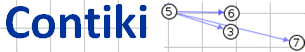
\includegraphics[width=2cm]{figs/contiki-logo.png}
	\hspace*{.5cm}
	
\includegraphics[width=2cm]{figs/tinyos-logo.jpg}
	\hspace*{.5cm}
	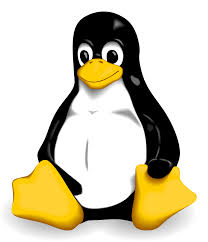
\includegraphics[width=2cm]{figs/linux-logo.jpeg}
	\hspace*{.5cm}
	
\includegraphics[width=2cm]{figs/riot-logo.png}
\end{frame}

%------------------------------------------------
\begin{frame}
	\frametitle{Overview of Closed Source OSes}
	\begin{columns}[c]
		\begin{column}{30cm}
			\vspace{.1cm}
			\begin{itemize}
				\justifying
				\item \textcolor{blue}{\href{https://mbed.org/}{ARM mbed}}
				\item Huawei LiteOS
				\item Google Brillo
			\end{itemize}
		\end{column}
	\end{columns}
	\vspace{.5cm}
	\hspace*{5.5cm} 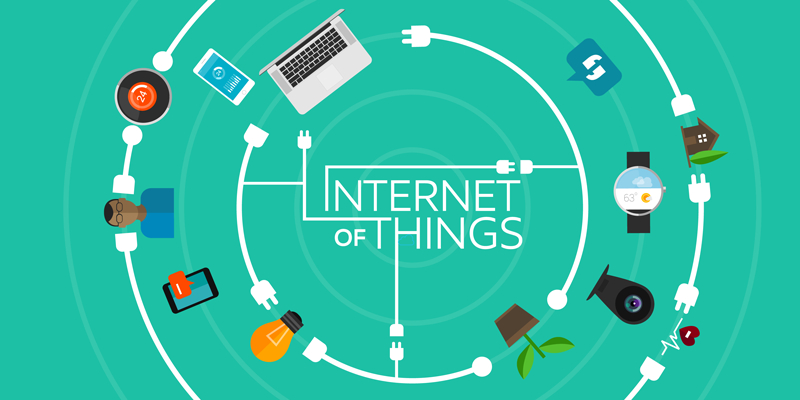
\includegraphics[width=5cm]{figs/Internet-of-Things-2.jpg}
\end{frame}

%------------------------------------------------
\begin{frame}
	\frametitle{ARM mbed}
	\begin{columns}[c]
		\begin{column}{30cm}
			\vspace{.1cm}
			\begin{itemize}
				\justifying
				\item Automation of power management
				\item Software asset protection and secure firmware updates for\\
				device security \& management
				\item Connectivity protocol stack support for Bluetooth® low energy,\\
				Cellular, Ethernet, Wi-fi, Zigbee IP, Zigbee NAN, 6LoWPAN
			\end{itemize}
		\end{column}
	\end{columns}
	\vspace{.5cm}
	\hspace*{5.5cm} 
\includegraphics[width=5cm]{figs/ARM-mbed-logo.png}
\end{frame}

%------------------------------------------------
\begin{frame}
	\frametitle{Huawei LiteOS}
	\begin{itemize}
		\justifying
		\item The company says that its \textcolor{TextOrange}{LiteOS} is the \textcolor{TextGreen}{lightest} software of its kind and can be used to power a range of smart devices
		\item There is another open-source ``LiteOS" project (UNIX-like OS for WSN). The relation between this \& that is not known.
		\end{itemize}
	\vspace{.5cm}
	\hspace*{5.5cm} 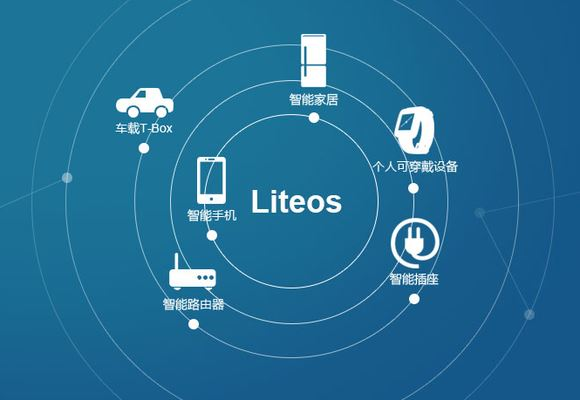
\includegraphics[width=5cm]{figs/huawei-liteos-logo.jpg}
\end{frame}

%------------------------------------------------
\begin{frame}
	\frametitle{Google Brillo}
	\begin{columns}[c]
		\begin{column}{30cm}
			\vspace{.1cm}
			\begin{itemize}
				\justifying
				\item Brillo is \textcolor{TextGreen}{derived} from Android
				but \textcolor{TextGreen}{polished} to just the lower levels.
				\item It supports Wi-Fi, Bluetooth Low Energy, and other Android things.
				\begin{itemize}
					\item Moreover, it will support the ``Weave" protocol
				\end{itemize}
			\end{itemize}
		\end{column}
	\end{columns}
	\vspace{.5cm}
	\hspace*{5.5cm} 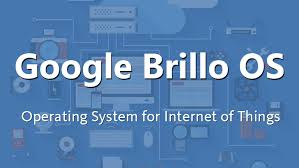
\includegraphics[width=5cm]{figs/google-brillo-logo.jpeg}
\end{frame}

%------------------------------------------------
\begin{frame}
	\frametitle{Why Not Linux?}
	\begin{columns}[c]
		\begin{column}{12cm}
			\vspace{1cm}
			\begin{block}{\centering\textcolor{darkred}{Real-Time Linux}}
				\justifying
				Controlling a laser with Linux is crazy, but everyone in this room is crazy
				in his own way. So if you want to use Linux to control an industrial welding
				laser, I have no problem with your using PREEMPT\_RT.
				\vspace{.2cm}
				\hspace*{9.5cm}\footnotesize{- Linus Torvalds}
			\end{block}
		\end{column}
	\end{columns}
	\vspace{.5cm}
	\hspace*{.5cm}
	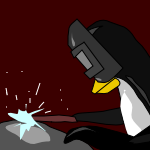
\includegraphics[width=2cm]{figs/preempt-rt.png}
	\hspace*{3cm}
	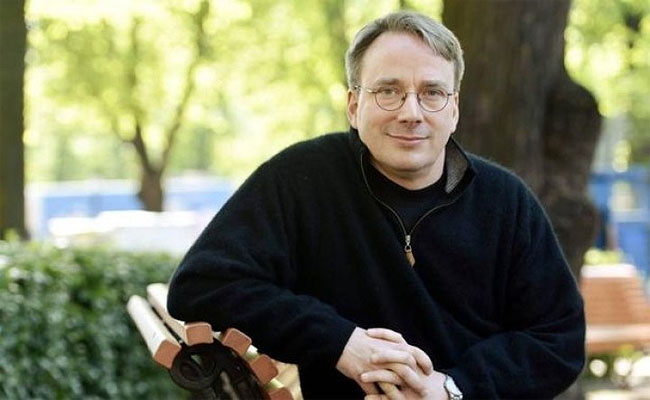
\includegraphics[width=5cm]{figs/linus-torvalds.jpg}
\end{frame}

%------------------------------------------------
\begin{frame}
	\frametitle{Why Not Linux?}
	\begin{columns}[c]
		\begin{column}{30cm}
			\vspace{.1cm}
			\begin{itemize}
				\justifying
				\item Linux certainly is a robust, developer-friendly OS
				\item Linux has a disadvantage when compared to a real-time operating system:
				\begin{itemize}
					\justifying
					\item Memory footprint
					\item It simply will not run on 8 or 16-bit MCUs
				\end{itemize}
				\item Linux will certainly have many uses in embedded devices, particularly\\
				ones that provide graphically rich user interfaces.
				\item There are thousands of applications for which Linux is ill suited.
			\end{itemize}
		\end{column}
	\end{columns}
	\vspace{.5cm}
	\hspace*{5.5cm} 
\includegraphics[width=5cm]{figs/tux-sad.png}
\end{frame}

%------------------------------------------------
\begin{frame}
	\frametitle{Outline}
	\begin{columns}[c]
		\begin{column}{30cm}
			\vspace{.1cm}
			\begin{itemize}
				\justifying
				\item \textcolor{LightGray}{Part I: IoT OS}
				\item Part II: IoT Protocol Stack
				\begin{itemize}
					\item Traditional Stack
					\item IoT Requirements
					\item IoT Stack
					\item Comparison
				\end{itemize}
				\item \textcolor{LightGray}{Part III: IoT Development}
				\item \textcolor{LightGray}{Conclusion}
			\end{itemize}
		\end{column}
	\end{columns}
\end{frame}

%------------------------------------------------
\begin{frame}
	\frametitle{Protocol stack}
	\begin{columns}[c]
		\begin{column}{30cm}
			\vspace{.1cm}
			\begin{itemize}
				\justifying
				\item<1-> Can you build an IoT system with familiar Web technologies?
				\item<2-> Yes you can, although the result would not be as \textcolor{Ocean}{efficient} as\\
				with the \textcolor{TextGreen}{newer protocols}.
			\end{itemize}
		\end{column}
	\end{columns}
\end{frame}

%------------------------------------------------
\begin{frame}
	\frametitle{Traditional Stack}
	\begin{columns}[c]
		\begin{column}{30cm}
			\vspace{.1cm}
			\begin{itemize}
				\justifying
				\item Existing Internet protocols such as HTTP and TCP are not optimized\\
				for very \textcolor{TextOrange}{low-power communication}.
				\item Energy is wasted by transmission of \textcolor{TextGreen}{unneeded data},
				\textcolor{TextGreen}{protocol overhead},\\
				and \textcolor{TextGreen}{non-optimized communication patterns}.
			\end{itemize}
		\end{column}
	\end{columns}
\end{frame}

%------------------------------------------------
\begin{frame}
	\frametitle{IoT Requirements}
	\begin{columns}[c]
		\begin{column}{30cm}
			\vspace{.1cm}
			\begin{itemize}
				\justifying
				\item A Low Power Communication Stack.
				\item A Highly Reliable Communication Stack.
				\item An Internet-Enabled Communication Stack.
			\end{itemize}
		\end{column}
	\end{columns}
\end{frame}

%------------------------------------------------
\begin{frame}
	\frametitle{IoT Stack}
	\begin{columns}[c]
		\begin{column}{30cm}
			\vspace{.1cm}
			\begin{itemize}
				\justifying
				\item \textsc{Low-Power Physical Layer} − \textcolor{TextOrange}{IEEE 802.15.4}
				\item \textsc{Power-Saving Link Layer} − \textcolor{TextOrange}{IEEE 802.15.4E}
				\item \textsc{Connecting To The Internet} - \textcolor{TextGreen}{IETF 6LoWPAN}
				\item \textsc{Routing} - \textcolor{TextGreen}{IETF ROLL}
				\item \textsc{Transport Layer and Above} - \textcolor{TextGreen}{IETF CoAP}
			\end{itemize}
		\end{column}
	\end{columns}
\end{frame}

%------------------------------------------------
\begin{frame}
	\frametitle{IoT Stack}
	\vspace{.25cm}
	\hspace*{.75cm} 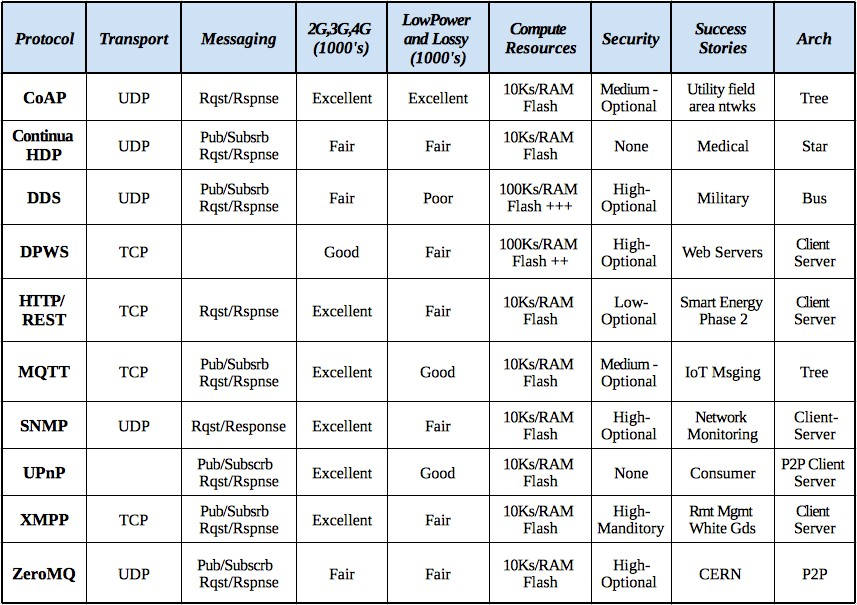
\includegraphics[width=10.5cm]{figs/iot-network-protocols.jpeg}
\end{frame}

%------------------------------------------------
\begin{frame}
	\frametitle{Comparison}
	\vspace{.5cm}
	\hspace*{1.5cm} 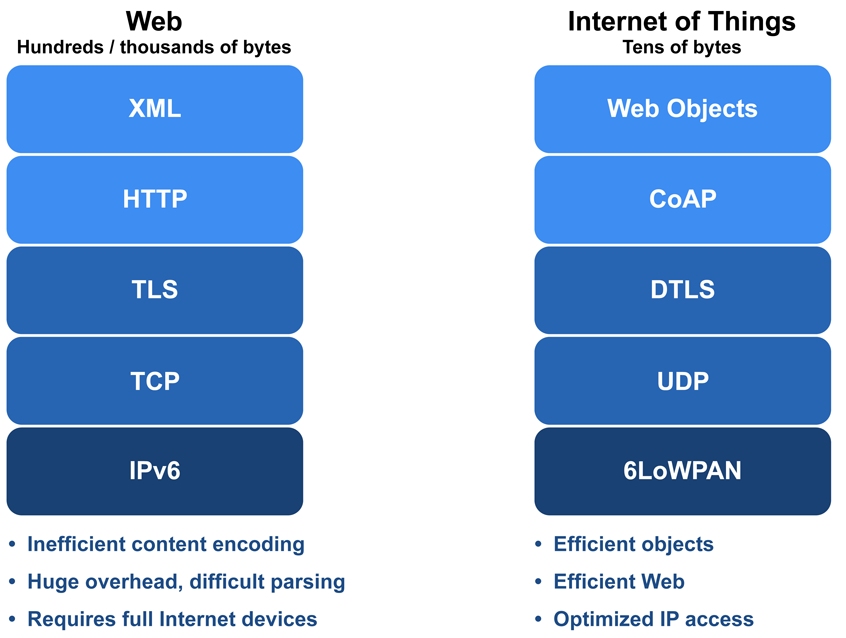
\includegraphics[width=10cm]{figs/Web-and-IoT-Stacks-1.png}
\end{frame}

%------------------------------------------------
\begin{frame}
	\frametitle{Comparison}
	\vspace{.5cm}
	\hspace*{.5cm} 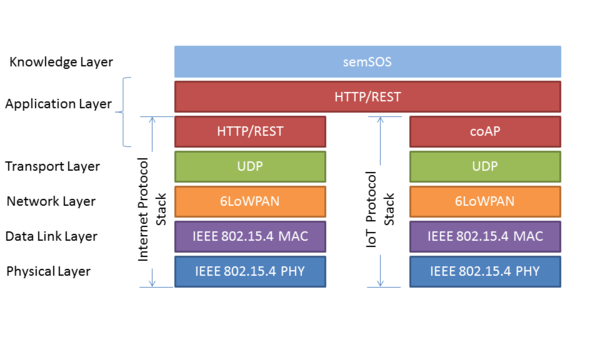
\includegraphics[width=12cm]{figs/Web-and-IoT-Stacks-2.png}
\end{frame}
%------------------------------------------------
\begin{frame}
	\frametitle{Outline}
	\begin{columns}[c]
		\begin{column}{30cm}
			\vspace{.1cm}
			\begin{itemize}
				\justifying
				\item \textcolor{LightGray}{Part I: IoT OS}
				\item \textcolor{LightGray}{Part II: IoT Protocol Stack}
				\item Part III: IoT Development
				\begin{itemize}
					\item The ``IoT-Lab" 
					\item RIOT environment
					\item Compilers
					\item Development environment
				\end{itemize}
				\item \textcolor{LightGray}{Conclusion}
			\end{itemize}
		\end{column}
	\end{columns}
\end{frame}

%------------------------------------------------
\begin{frame}
	\frametitle{The ``IoT-Lab"}
	\begin{itemize}
		\justifying
		\item IoT-LAB provides a very large scale infrastructure suitable for testing small wireless sensor devices and heterogeneous communicating objects
		\item IoT-LAB provides full control of network nodes and direct access to the gateways to which nodes are connected, allowing researchers to monitor nodes energy consumption and network-related metrics.
	\end{itemize}
	\vspace{.5cm}
	\hspace*{5.5cm} 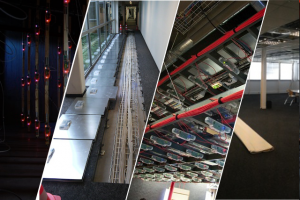
\includegraphics[width=5cm]{figs/iot-lab-1.png}
\end{frame}

%------------------------------------------------
\begin{frame}
	\frametitle{The ``IoT-Lab"}
	\begin{center}
	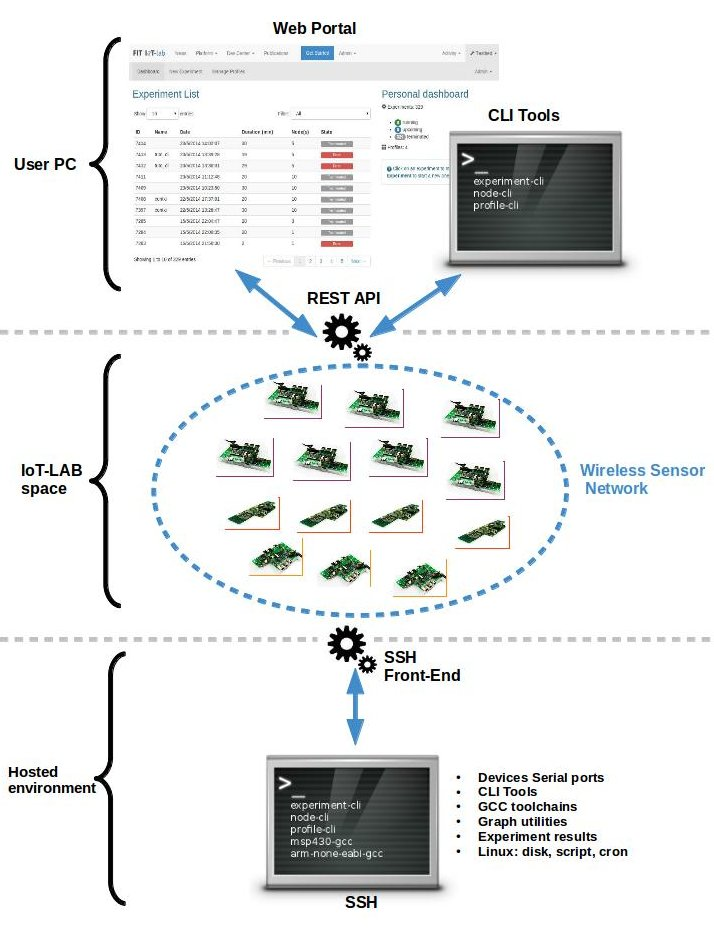
\includegraphics[width=6cm]{figs/IoTLab-platform-overview.jpg}	
	\end{center}

\end{frame}
%------------------------------------------------

\iffalse
%------------------------------------------------
\begin{frame}
	\frametitle{A scientific testbed}
	\begin{columns}[c]
		\begin{column}{30cm}
			\vspace{.1cm}
			\begin{itemize}
				\justifying
				\item IoT-LAB provides full control of network nodes and direct access\\
				to the gateways to which nodes are connected, allowing researchers\\
				to monitor nodes energy consumption and network-related metrics.
			\end{itemize}
		\end{column}
	\end{columns}
	\vspace{.5cm}
	\hspace*{5.5cm} \includegraphics[width=5cm]{figs/iot-lab-1.png}
\end{frame}
\fi
%------------------------------------------------
\begin{frame}
	\frametitle{The ``IoT-Lab" topologies and environments}
	\vspace{.1cm}
	\begin{itemize}
		\item IoT-LAB testbeds are located at six different sites across France which 
		gives forward access to \textcolor{TextOrange}{2728 wireless sensors nodes}.
	\end{itemize}
	\vspace{.5cm}
	\begin{itemize}
		\item 512 WSN430 Node (800MhZ)
		\item 632 WSN430 Node (2.4GhZ)
		\item 938 M3 Node
		\item 550 A8 Node
		\item 96 Open Host Node		
	\end{itemize}
\end{frame}

%------------------------------------------------
\begin{frame}
	\frametitle{The ``IoT-Lab" Different nodes}
	\vspace{.1cm}
	\begin{itemize}
		\item The IoT-LAB hardware infrastructure consists of a set of IoT-LAB nodes.
		\item A global networking backbone provides power and connectivity to\\
		all IoT-LAB nodes and guaranties the out of band signal network\\
		needed for command purposes and monitoring feedback.
		\item Nodes' Operating Systems
		\begin{itemize}
			\item Contiki
			\item RIOT
		\end{itemize}
	\end{itemize}
	\vspace{.5cm}
	\hspace*{5.5cm} \includegraphics[width=4cm]{figs/iot-lab-2.png}
\end{frame}

%------------------------------------------------
\begin{frame}
	\frametitle{The ``IoT-Lab" A part of FIT}
	\vspace{.1cm}
	\begin{itemize}
		\item IoT-LAB is a part of the FIT (Future Internet of the Things) platform.
		\item FIT is a set of complementary components that enable experimentation
		on innovative services for academic and industrial users.
	\end{itemize}
	\vspace{.5cm}
	\hspace*{5.5cm} \includegraphics[width=5cm]{figs/iot-lab-4.png}
\end{frame}

%------------------------------------------------
\begin{frame}
	\frametitle{The ``IoT-Lab" Experiments}
	\vspace{.1cm}
	\begin{itemize}
		\item you can setup an experiment in
		\href{http://iot-lab.info}{\textcolor{blue}{``IoT-Lab" website}} with following
		features:
		\begin{itemize}
			\item Experiment duration
			\item Node Architecture
			\item Node Host Lab
			\item Node numbers
		\end{itemize}
		\item Later you can setup test profile and upload your framework for your specific node.
	\end{itemize}
	\vspace{.5cm}
	\hspace*{5.5cm} \includegraphics[width=5cm]{figs/iot-lab-3.png}
\end{frame}

%------------------------------------------------
\begin{frame}
	\frametitle{Arduino Platform}
	\vspace{.1cm}
	\begin{itemize}
		\item One of the best-known names among open source IoT projects.
		\item Arduino is a platform that encompasses both hardware and software.
		\item The software includes an integrated development environment (IDE) for writing code in the Arduino language that just like C.
	\end{itemize}
	\vspace{.5cm}
	\hspace*{5.5cm} \includegraphics[width=5cm]{figs/Arduino-Logo.png}
\end{frame}

%------------------------------------------------
\begin{frame}
	\frametitle{IoT Toolkit}
	\vspace{.1cm}
	\begin{itemize}
		\item The Internet of Things today consists of many different sensor networks and protocols, connected to dedicated cloud services, providing access through smartphone and browser apps. It is rare for these separate "silos" to cooperate or interact with each other.	
	\end{itemize}
	\vspace{.5cm}
	\hspace*{2cm} \includegraphics[width=10cm]{figs/iot-toolkit-2.jpg}
\end{frame}

%------------------------------------------------
\begin{frame}
	\frametitle{IoT Toolkit}
	\begin{itemize}
		\item The IoT Toolkit is an Open Source project to develop a set of tools for building multi-protocol Internet of Things Gateways and Service gateways that enable horizontal co-operation between multiple different protocols and cloud services.
	\end{itemize}
	\vspace{.1cm}
	\hspace*{3cm} \includegraphics[width=8cm]{figs/iot-toolkit-1.png}
\end{frame}

%------------------------------------------------
\begin{frame}
	\frametitle{webions}
	\begin{itemize}
		\item Webinos is a web-based application platform for the internet of things.
		\item The \textbf{webinos} project will define and deliver an Open Source Platform and software components for the Future Internet in the form of web runtime extensions, to enable web applications and services to be used and shared consistently and securely over a broad spectrum of converged and connected devices.
	\end{itemize}
	\vspace{.1cm}
	\hspace*{3cm} \includegraphics[width=8cm]{figs/webinos-logo.png}
\end{frame}

%------------------------------------------------
\begin{frame}
	\frametitle{RIOT environment}
	\vspace{.1cm}
	\begin{itemize}
		\justifying
		\item RIOT features the native port with networking support.
		\item This allows you to run any RIOT application on your Linux or Mac computer and setup a virtual connection between these processes.
	\end{itemize}
	\vspace{.5cm}
	\hspace*{5.5cm} \includegraphics[width=5cm]{figs/riot-logo.png}
\end{frame}

%------------------------------------------------
\begin{frame}
	\frametitle{Compilers}
	\vspace{.1cm}
	\begin{itemize}
		\justifying
		\item Family: ARM
		\begin{itemize}
			\item gcc-arm-embedded toolchain
			\item CodeBench toolchain
			\item Linaro toolchain
		\end{itemize}
		\item Family: ATmega
		\begin{itemize}
			\item Atmel AVR Toolchain
		\end{itemize}
		\item Family: MSP430
		\begin{itemize}
			\item MSPGCC toolchain
		\end{itemize}
	\end{itemize}
	\vspace{.5cm}
	\hspace*{5.5cm} \includegraphics[width=5cm]{figs/parse-tree.png}
\end{frame}

%------------------------------------------------
\begin{frame}
	\frametitle{ARM: gcc-arm-embedded toolchain}
	\vspace{.1cm}
		\begin{itemize}
			\justifying
			\item ARM is maintaining a GNU toolchain with a GCC source branch targeted at Embedded ARM Processors, namely Cortex-R/Cortex-M processor families	
		\end{itemize}
	\vspace{.5cm}
	\hspace*{5.5cm} \includegraphics[width=5cm]{figs/CompilerAssemblerToolchain_gcc.png}
\end{frame}

%------------------------------------------------
\begin{frame}
	\frametitle{Development environment}
	\vspace{.1cm}
	\begin{itemize}
		\justifying
		\item Most of the IoT OS developed on \textcolor{TextOrange}{Linux} and\\
		use \textcolor{TextGreen}{traditional make} as build system.
	\end{itemize}
	\vspace{.5cm}
	\hspace*{.5cm}
	\includegraphics[width=5cm]{figs/linux-logo.jpeg}
	\includegraphics[width=5cm]{figs/gun-logo.png}
\end{frame}

%------------------------------------------------
\begin{frame}
	\frametitle{Outline}
	\begin{columns}[c]
		\begin{column}{30cm}
			\vspace{.1cm}
			\begin{itemize}
				\justifying
				\item \textcolor{LightGray}{Part I: IoT OS}
				\item \textcolor{LightGray}{Part II: IoT Protocol Stack}
				\item \textcolor{LightGray}{Part III: IoT Development}
				\item Conclusion
				\begin{itemize}
					\item Summary
					\item Open problems
					%\item Event-Driven, Non-Blocking I/O Model
				\end{itemize}				
			\end{itemize}
		\end{column}
	\end{columns}
\end{frame}

%------------------------------------------------
\begin{frame}
	\frametitle{Summary}
	\begin{itemize}
		\justifying
		\item Different applications of IoT $\Rightarrow$ Different OS Requirements (e.g., Energy, Memory, Realtime, ...) $\Rightarrow$ Different OSes
		\item A few OSes should be examined
		\item In the next step, we want to develop an evaluation environment and focus on RIOT 
		\begin{itemize}
			\item We have already enough experience on Linux 
		\end{itemize}
		\end{itemize}
\end{frame}


%------------------------------------------------
\begin{frame}
	\frametitle{Open problems}
	\begin{columns}[c]
		\begin{column}{30cm}
			\vspace{.1cm}
			\begin{itemize}
				\justifying
				%\item Ideally, the capabilities of a full-fledged OS should be available on all IoT devices.
				\item Native Multi-Threading
				\item Hardware Abstraction
				\item Dynamic Memory Management
				\item Fulfill Strict Energy Efficiency
			\end{itemize}
		\end{column}
	\end{columns}
	\vspace{.5cm}
	\hspace*{5.5cm} \includegraphics[width=5cm]{figs/open-problems.jpg}
\end{frame}

%------------------------------------------------
\iffalse
\begin{frame}
	\frametitle{Event-Driven, Non-Blocking I/O Model}
	\begin{columns}[c]
		\begin{column}{30cm}
			\vspace{.1cm}
			\begin{itemize}
				\justifying
				\item Networking Event-Driven
				\item Non-Blocking I/O
			\end{itemize}
		\end{column}
	\end{columns}
	\vspace{.5cm}
	\hspace*{5.5cm} \includegraphics[width=5cm]{figs/io.png}
\end{frame}
\fi
%------------------------------------------------
\begin{frame}
	\vspace{1cm}
	\begin{Huge}
		\begin{center}
			\usebeamercolor[fg]{title}Questions?
		\end{center}
	\end{Huge}
\end{frame}

%------------------------------------------------
\begin{frame}
	\frametitle{Multi-Tasking, Thread Model (IoT OS)}
	\begin{columns}[c]
		\begin{column}{30cm}
			\vspace{.1cm}
			\begin{itemize}
				\justifying
				\item Most RTOS products on the market are thread model.
				\item \textcolor{TextGreen}{Tasks} are now called \textcolor{TextGreen}{threads}.
				\item All the \textcolor{TextOrange}{tasks} code and data occupy
				\textcolor{Ocean}{the same address space},\\
				along with that of the RTOS itself.
				\item Or every \textcolor{TextOrange}{tasks} can run in its own thread and \\
				\textcolor{Ocean}{has its own memory stack}.
			\end{itemize}
		\end{column}
	\end{columns}
	\vspace{.5cm}
	\hspace*{5.5cm} \includegraphics[width=3.5cm]{figs/thread-model.jpg}
\end{frame}

%------------------------------------------------
\begin{frame}
	\frametitle{Multi-Tasking, Process Model (IoT OS)}
	\begin{itemize}
		\justifying
		\item By using the MMU, each task (now called a process) occupies its own private address space
		\item This model has the great benefit that each process has no access to, or even awareness of, other processes’ memory or that of the OS itself
		\item The memory needs to be remapped using the MMU
	\end{itemize}
\end{frame}

%------------------------------------------------
\begin{frame}
	\frametitle{What are the main components in IoT OS}
	\begin{columns}[c]
		\begin{column}{30cm}
			\vspace{.1cm}
			\begin{itemize}
				\justifying
				\item Networking
				\item Memory Manager
				\item Task Scheduler
			\end{itemize}
		\end{column}
	\end{columns}
\end{frame}

%------------------------------------------------
\begin{frame}
	\frametitle{OS Classification}
	\begin{columns}[c]
		\begin{column}{30cm}
			\vspace{.1cm}
			\begin{itemize}
				\justifying
				\item Programming Model for an IoT OS
				\begin{itemize}
					\item All tasks are executed within the same context and have\\
					no segmentation of the memory address space.
					\item Every process can run in its own thread and has its own\\
					memory stack.
				\end{itemize}
			\end{itemize}
		\end{column}
	\end{columns}
\end{frame}

\end{document}
